\documentclass[12pt]{article}

%\usepackage{afterpage}

%\usepackage{pdflscape}
\usepackage{lscape}


\usepackage{geometry}
\geometry{a4paper,left=10mm, right=10mm, top=20mm, bottom=20mm}

\usepackage{graphicx}
\graphicspath{ {images/} }

\usepackage{tabularx}
\usepackage{colortbl}

\usepackage{fancyhdr}
\fancyhf{}
\lhead{Escort The President}
\rhead{Final Report}
\rfoot{Page \thepage}

\usepackage{enumitem}

\newcommand{\nl}{\newline\vspace*{1 cm}\newline}
\newcolumntype{Y}{>{\centering\arraybackslash}X}
\newenvironment{lst} {\vspace{-5mm}\begin{enumerate}[label =\arabic*]} {\vspace{-\topsep}\end{enumerate}}

\newcommand{\f}{\cellcolor{black}}
\newcommand{\return}{\\\\\noindent}
% You must use this in a subsubsection.
\newenvironment{req} {\begin{enumerate}[leftmargin=2.5cm, label = \textbf{REQ \arabic{subsection}.\arabic{subsubsection}.\arabic*:}]} {\end{enumerate}}

\title{
\includegraphics[scale=1]{final-report-logo}\\
\Huge\textbf{Final Report}}

\author{Ahmed Bhallo \and James Birch \and Edward Dean \and Brendan Hart \and Kwong Hei Tsang}

\date{\today}

\begin{document}
\maketitle

\begin{abstract}
This is the final report for our game, Escort The President. This document will detail the design and implementation process, and how we worked as a team. We have included the requirements and documented changes made from the specification.\return
Escort The President is a competitive multiplayer game where each rounds consists of assassins attempting to assassinate the recently elected president. Assassins carefully plot their move to kill the president. Gunshot! An assassin has shot at the president and the president's escorts (with the aid of police officers) attempt to escort him to the safezone alive. To make matters worse, this is in public streets and there are civilians everywhere! 
\end{abstract}

\newpage
\pagestyle{fancy}
\tableofcontents
\newpage

\section{Introduction}
This report will talk about the design and implementation process that we followed in producing our videogame, Escort The President. This will include the features we included in the game, the software engineering behind it and also to discuss the teamwork aspect of the project and how we worked together to make the game a reality.\return
For this project, we received a brief which stated that we must make a videogame that contains the following 5 features:
\begin{enumerate}
\item \textbf{Competitive play.} Your game must allow players to compete.
\item \textbf{Networking.} Your game must allow multiple players to play across a network. The specific net-
working arrangement depends on the type of game but, for example, you might create a client-server type
arrangement in which multiple clients connect to a controlling server, or a server performing some other
service.
\item \textbf{Artificial Intelligence.} Your game must have the option of computer-controlled players. These might
be individual or team players, depending on the type of game.
\item \textbf{User Interface.} Your game must have a user interface, i.e. a convenient way for players to interact
with the game. This will almost certainly require a menu as a minimum but will more than likely also
require other interface entities such as dialog windows that have a range of controls, clickable icons, etc.
The user interface will also include crucial feedback information for the player.
\item \textbf{Audio.} Your game should include audio in the form of music and spot effects, as a minimum.
\end{enumerate}
This was a bare minimum, though, and we knew from the start that we wanted to create something that was much more about imagination and creating a fun game than it was to simply just 'make a game'.\return
As soon as the idea of this game was mentioned and ideas about how it could work started to form, the more excited we got about the concepts and we quickly had a goal where everyone was on board and committed to making it happen.\return
The game we have built comprises of a blend between custom components built by the team (such as the User Interface) as well as also using tried-and-testing algorithms for other aspects (such as A* for AI route finding) to create a game that fits into an enjoyable genre of retro shooters while introducing some originality too.\return
This report will cover in detail the process we followed to achieve this and will discuss the design of the game's features, how our requirements specification is reflected in the product, the software engineering principles we followed to improve the quality of the output, how we mitigated risk throughout the lifetime of the project and also how teamwork allowed us to create what we have today. A full evaluation and reflection is also provided accompanied with an individual report on our own personal experiences for this endeavour.
\newpage
\section{Final Requirements}
During the implementation phase of the game, we decided that some of the requirements that we had sought to implement did not meed with our expectations of the game. As a result, these requirements were removed or modified to make our game more enjoyable. During team discussions, we also decided to formalise in the form of requirements all the non-functional requirements that will ensure our system is secure and robust. More importantly, we documented measures to prevent malicious clients and cheaters.
\subsection{Design changes and Balancing}
Our ultimate goal was to ensure that Escorts and Assassins always win roughly half the time. All design and balance changes were made to help achieve this goal.\return
During play testing, we realised that our initial values for weapon damage was too overpowered, making it very easy to die. For instance, it would only take 2 bullets to kill an Assassin. As a result, we decided to change the damage of bullets, and also give Assassins more health to match with Escorts' health. We also noticed that it is very hard for Escorts to win a game because the President would die too quickly. After a lot of testing, we found that 800 health for the president was a good value as it was slightly harder for Assassins to win, but easy enough so that Assassins will win roughly half of the time. Another additional advantage we gave to Escorts was increasing the health of a blast shield. Even though Assassins also have blast shields, we felt that blast shields were a staple to Escorts who are more of a defensive team and would therefore use it more.\return
Our original design had Menaces in the game -- Assassins who have recently killed civilians. Being a Menace meant that one could now attack Assassins, and Assassins could attack back. We felt that this was a bad game design decision, as the Assassins were essentially a team -- They won together, and lost together. Their shared the same goal of killing the president so it did not make any sense for them to fight each other. Thus, we removed Menaces from the game. To give Civilians more of a purpose as a result of this, Escorts can now shoot Civilians to give the game more of a chaotic feel, and also to make the role of a Civilian more of a nuisance that absorbs bullets.\return
When a unit dies, we decided not to have the unit drop their left over ammo and grenades. This is due to that we have power up that adds grenades and extra magazine anyway. So having this feature would have introduced too much ammunition and grenades.\return
We didn't include super power ups because it would have made the game to unbalanced. The player that would pick up one of these would have been too overpowered.\return
We intended having 20 civilians in the game but we found that this created a lot of lag and made the game less enjoyable. So we reduced it to a maximum to 5. The civilians can be changed before the game has started from 0 to 5 civilians.\return
We decided to reduce the hit points of the blast shield by half because during game play you could run the president to the safe zone without death and in turn making it impossible for the assassins to kill the escorts.\return
We also felt it would be in the interest of the game to remove the scoreboard and Kill/Death ratio features. This is because we thought that it may incentivise the players to try and focus more on simply killing each other to get the biggest scores whereas completing the objective is a much more important aspect of this game than it being an out-and-out deathmatch.
\subsection{Malicious clients}
We have considered cheaters in our game and implemented cheat prevention mechanisms. This mean that players can throw grenades if they don't have any grenades left even if they spoof the packets to throw a grenade. This is the same for shooting. When the server receives a message from the client, the server check if the player can do whatever it needs to do as the client will only send an action not the result of the an action. So the server will execute the action and send the result to the client. In addition to the game itself, similar mechanism is also applied on the operations on lobbies. Constraints are always checked to prevent unexpected behaviour from occuring on the server due to inconsistent data, such as a player can only create a new lobby when he/she is not in one, player cannot join a lobby when he/she is in one already until leaving current lobby.
\newpage
\section{User Experience}
We've put a lot of effort into ensuring our product has an excellent UI-UX. Our menus went through multiple iterations and changes after feedback from the team and other users who tried using them. We believe that any inconsistency in the UI would throw the users off. For instance, when a user sees a menu with a certain look-and-feel, they will expect the same look-and-feel when they are in game. Using a built in library such a JavaFX would go against this as you do not have direct control over the components (when overlaying them directly over the game). As a result, we decided to create our own components that would be used in menu and in game.\return
The components are detachable from our game, so this will allow reuse for any Java product with no changes necessary. We following the "You aren't gonna need it" principle, thus only creating components that we actually needed and will be used and included in the final product. However, components are also very extensible to changes and new types of components can very easily be built on top of the already existing set of components.
\subsection{User Interface}
We followed the "less is more" principle when designing our menus. For connecting to a server, we decided to only include the bare minimum for what a user needs to enter to connect to the server. This will mitigate the likelihood of the user feeling overwhelmed. The same principles were followed throughout all the menu sections. For when displaying a list of the lobbies on the server, we decided for the client to automatically request a refresh from the server every 3 seconds. As well as not having a manual refresh button, our idea was to obfuscate the refreshing away from the user. All they need to do is find a lobby they want to join, and also filtering lobbies they don't like.\return
We have included a settings menu that allows users to change their environment to their liking. Users can change the the resolution of the game depending on their display monitor. The game also detects the resolution of the screen automatically. Users can select between fullscreen and windowed mode. We have provided users the option to change the volume of the music and sound effects or fully mute either. Users can also change the key bindings of all keys in the game to allow players to change what keys they like to use.
\subsection{Heads-up display}
For the in-game HUD, we decided to keep it very simple and only include necessary information to the user as to not make them feel overwhelmed. We included the mini-map; in-game chat; weapons panel (when the client is alive); and spectating panel (when the client is spectating).\return
From experience, we have noticed some chat boxes from other products that make it very hard to scroll up and review old messages while new messages are still being added. We took this into account, and only move the scroll bar to the bottom when it is already at the bottom.\return
We have included a radar in our game to allow users to see all players on the map. To help accommodate users with poor eyesight, we ensured that the pixels indicating player location on the map were big enough to see by people of all ages.\return
At at the top of the screen, we includes a heads up display that shows how much ammo you have left, how many grenades and your blast shield hit points left. Furthering the less is more idea, when a user is dead, we remove the weapons panel as this may cause some confusion at first (seeing as it is no longer in use)\return
For the spectator system, the UI was designed to allow the player to easily view the unit that's currently being spectated, as well as providing a UI which does not obstruct this view. We chose the best way to do this was a simple box towards the top of the screen to display the username currently being spectated and buttons either side to indicate which direction they are changing the currently spectated unit in. This allows the player to easily scroll through the units until they find one which interests them. The player is also presented with the time left until respawn, so they can adequately prepare and focus for their next period of play.
\subsection{Graphics}
We have decided to go for a 2.5D top-down perspective, but not a direct bird's-eye view in order to give depth to boundaries such as walls. This will grant players the freedom to move in 8 directions and feel in control of their unit. The game will only have 2 layers of depth (in order to not be confusing) �?The ground tiles (the floor), and the obstacle tiles (think of boxes and walls placed on the ground that are the size of a character). We could have chosen to design the game in 2d but we didn't feel that the game would have been engaging enough for the type of game we are designing.\return
We've created our own pixelated sprites to give the users of a game a nostalgic feel. We believe that this was our best options as it not only looks good, but also easy to draw. We created tiles in the same way but with a higher resolution so that characters stand out more.\return
We used Graphics2D to stick to a graphics library already built into Java. There a lot of method that are helpful such as getting the screen resolution so can scale properly to fit your screen size. We could have used other graphics libraries that would have been faster. But as our team was inexperienced in writing a graphic user interface, we stuck with the basics.\return
As our game is very pixilated and blocky, we had to design music that fitted with the theme. So the obvious choice was to create 8 bit like music and sound effects. This made the game feel more retro and having the arcade-sounding sound effects and chiptune music made the game more immersive and engaging. We create our own music and sound effects from scratch to exactly fit the theme of our game.\return
During game play, the camera will follow you around the map. But we have also included a feature to the camera that allows you to freely move it around the map to see what is going on. To do this, you press the "Y" key (or what you have bound to it) and you can use the mouse to move the camera around. By moving the mouse to the edges of the screen the camera will follow and move in that direction.\return
\newpage
\section{Game Design}
\subsection{Movement}
When the creator of Super Mario Bros, Shigeru Miyamoto, was asked why the Mario franchise was so popular, he talked about the way they implemented movement. One element of Mario’s movement was his slide (he doesn’t stop moving exactly when a button is released). This made the movement feel more natural, making our players feel immersed into the game.
\subsection{Combat system}
We decided to include the use of grenades in our game as this would allow the players to have a variety of damaging weapons at their disposal. It also introduced an area of effect damage so a player is able to deal damage to a area of players.\return
We have included a blast shield that reduces damage from damaging weapons. The blast shields will stop bullet damage completely where it only stops 80\% of grenade damage. The shield can be use for a tactical advantage where if the reloading time will kill you and you need to make a retreat, the shield would be a good choice.\return
We have decided for the pistol to have unlimited ammo as all player should have a weapon that they can use and not feel empty.\return
We have include a weapon type choice in our game to give more of a variety of gameplay that the user can experience. This pistol is a semi-automatic weapon where the machine gun is a fully automatic weapon.
\subsection{Power Ups}
We have added power ups to the game so that it makes the game more interesting. It can provide a second change to a player if the run out of ammo or have very little health. This can make the game last longer and provide more entertainment. To pick up a power up, you just walk over it. We included a time out for the power ups so that they disappear after a set time to prevent spamming. Is also reduced the effectiveness of power ups as not all of them are active so will have to rely on the skills of the player.
\subsection{Map Creator}
We have created the map load so that it takes an images and each pixel represents a tile. This also allows other people to create their own map by drawing one, all you need is a simple image editor like paint to create these images and then load them into the game.
\subsection{Unit Assignment}
If you are the only player, you will always be assigned an escort because there must always be one escort to protect the presidents and lead him to safety. When there are more players, overall there will be more assassin's than escorts as there is an advantage to the escort side than the assassin side. This is due to that the president has many police ai around him all the time so need to defeat the police and escorts to then attack the president. This assignment is random so that players can get a chance of player on the opposite side.
\subsection{Leaving a Game}
When a user leaves the game they are replaced by an AI controller to ensure that the number of players on each side is kept balanced.
\subsection{President Following}
The President's AI was kept simple so not to over complicate things. The President only moved when an escort came close enough and pressed the 'F' key (or what the player bound to the follow key). This allows an easy implementation as some of our other ideas were quite complex. When the escort dies, the President will just stand and not move because of the way we implemented the following system, as we assume that President is defenceless and relied on the escorts and police to protect him.
\subsection{AI}
We decides that the ai shouldn’t be on point every shoot so decided to give the ai a slight inaccuracy to the shooting to give the ai more of a human like shooting effect and less robotic and cheaty.\return
To add to the feel of the game, we include civilians to the game. These just wander around and do nothing toward completing the game. This just give the added feel to the game that there are people to look out for. This also has the added benefit that it fills the map up with extras so not to feel so empty when playing. You could also think that if this would happen in real life, there would be people around in panic as well.
\subsection{Spectating}
We have include a respawn time when you die so during this time of waiting we have implemented a spectator system that allows you to see what other players are doing. Also it gives you something to do whilst you wait. You can cycle through your team and the opposite team so to compose yourself and gain insight in what the other team might do.
\newpage
\section{Software Design}
The software is split into a few major components, each of them are responsible for a major type of operations:
\begin{enumerate}
\item Network: maintaining client connections and transmitting messages over the network
\item Client UI: interacting with the player
\item Lobby Management: gathering players for a game and chat messages
\item Server Console: administrative operations on the server
\item Game Logic: executing updates and enforce game rules in the game state during the game
\end{enumerate}
{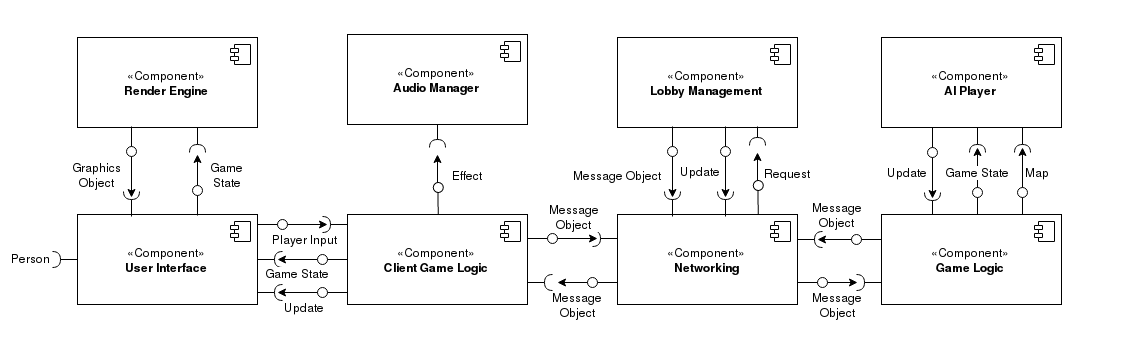
\includegraphics[width=550px,height=\textheight,keepaspectratio]{component_diagram}}

\begin{enumerate}
\item Structural pattern: Interface instead of concrete classes are used to interact between different some classes so that they are less dependent on each other. For example, message control interface is used instead of using sockets directly when dealing with messages so that different communication methods can be implemented without changing the rest of the components.
\item Executing pattern: Objects in Lobby Management are synchronized so that it is thread-safe as there may be a lot of clients requesting updates on the lobbies on the server. Game logic uses a game loop with regular refresh period to do correct timing so that the state is updated correctly and thread safe.
\end{enumerate}
\subsection{Game logic} 
Items in the game such as weapons, entities, AI controllers are separated into different classes so that the handle exactly one item. Requests from players and AIs are processed by a Game Message Queuer and updates executed by the game loop in the Game thread by calling methods of each objects that need to be updated.

\subsection{Networking}
Tasks are different in each class. Player thread is for distinguish message types and do the correct requests to different components such as \texttt{ServerSide} object handling server environments, lobby management object handling lobby related requests and game logic for requests in the game. Server object is for handling incoming connections and packets from the network. \return
A major change in networking is the choice of underlying communication protocol. TCP connections remain the same as in the specification. For UDP, instead of implementing protocols for packet loss handling, TCP is used instead for critical messages and UDP for others, to reduce the complexity of the code and less debugging by utilizing existing libraries.
\subsubsection{Protocols}
We used the TCP and UDP protocols because it is a common standard that most programs and game use these days so will be suitable. This will also make the game work in most network environments.
We used TCP because it provides a mechanism to guarantee any messages sent between server and the client reaching each other. Libraries for encryption are also ready for use to secure the data sent between the server and client. It is useful if the client is connecting through an insecure network such as public WiFi or a restrictive network which prevents UDP from working properly.
We also decided to include the use of UDP because it gives us The benefit from it is not all lost messages have to be resent as they may be out of date such as the game state. This allows server and client to selectively resend important lost information only, increasing efficiency. At the same time, it reduces handshaking to reduce the delay. This made it useful when the player is far away from the server or is connecting through a trusted network. But UDP does have its drawbacks sudo as that it doesn’t guarantee each packet can reach each side as packet loss are not handled by the protocol.
\subsubsection{Encryption}
We have used TLS to encrypt our traffic because it prevents attackers from man in the middle attacking our connection and so not being able to change the packets. This provides a more secure game and ensure that the players get a smooth game without the worries of being interfered.
\subsection{Lobby Management}
Lobby objects are used to wrap the list of players, lobby ID, password and settings. \texttt{LobbyManagement} class is for checking constraints, executing updates for a lobby and notify clients and also game starting when a corresponding valid request is received.

\subsection{Cheat prevention}
Constraints are checked in each component before processing any messages from the network because it may be malicious. We will always identify the actual identity of the player by its connection and also verify whether the message is properly formed so that the server won't get screwed up when an invalid request is received. For example, a player is not allowed to send any message as another player because connections are TLS encrypted and the server will overwrite the identification information with the one found on the server based on the connection. The same applies to lobby management as well including verifying the requests is coming from master and target is in the same lobby before executing kicking, play name spoofing protection in lobby messages.
\newpage
\section{Software Engineering}
\subsection{Planning}
After deciding on the idea for our game, we attempted to further define our game through the use of a variety of strategies. The idea was that with these strategies combined we would have a firm idea of what needs to be done at the start of development as well as throughout the entire project.
\subsubsection{UML Diagrams}
We utilised UML to decide which components were necessary and how they should work together. The UML diagrams considered the communication between these components and also aided in splitting these components into smaller tasks. Doing this instilled some clarity in how we should implement our ideas and make it clear between members of the team how a particular feature should be implemented. We found it useful to draw rough sketches of UML during our meetings when we were together as we found it easier to discuss some more complex processes in person where we could draw ideas out for each other. 3 Use Case Descriptions for shooting, changing client resolution and joining a private lobby can be found in Appendix C.
\subsubsection{Trello Board}
We made use of a Trello board. This is an online tool which acts as a 'noticeboard' where teams can write out tasks and other members can view these. Everyone in a team can then comment on these tasks and tasks can be assigned along with deadlines. This allowed us all a platform to add tasks which are grouped together, so we could all have a visual representation of what needs to be done, as well as what we may be missing. However, as the project wore on (and features were being completed) our use of this tool waned and we opted for talking on instant messenger as an easier way to inform each other of progress.
\subsubsection{Gantt Chart}
We also created a Gantt chart. The purpose of this was to aid in assigning tasks to the team and attempt to set start and end dates on each task. This allowed us to visually see what is expected of us by a certain date, and begin planning in advance. At the start, we found it quite easy to follow this plan but as more of the project was being completed, it started becoming apparent that it would be too difficult to follow the Gantt chart faithfully. This was due to some tasks being completed quicker and others longer than anticipated. This resulted in members of the team needing to be flexible to help each other out and to plug any gaps to make sure that we did not fall too far behind when tasks were building up.
\subsubsection{Sprint Plans}
Since we decided to operated in week-long sprints, we decided on creating week-long plans so we could see what is expected in the short term. These plans were inspired by the Gantt chart, but were driven by the current progress in the development of the game so were often more useful than the Gantt chart. These plans were usually informal notes taken during meetings once-per-week and gave each member of the team a chance to share what they had completed in the week just gone and what they should aim to have completed by next week. Honesty was key in these sessions so that task progress could be judged by the team. We noticed that having this mix between meeting in person and discussing over instant messaging to be well-balanced because it meant we could have some freedom to work on tasks in our own time (while being able to still contact the team) but also when we needed to come together and be in a focussed environment then we could do.
\subsection{Principles of Development}
Throughout the development of our game, we have attempted to follow various principles of development in the hope that this will produce code which is of high quality and easily maintainable.
\subsubsection{Don't Repeat Yourself}
One of these principles was Don't Repeat Yourself (DRY). This involves ensuring that code which may be duplicated is put into methods which are called in multiple places to reduce the need to copy and paste code. The advantage of this is that any changes that need to be made to this code only need to be made in one place, making bug fixes easier as well as testing. We managed to follow this principle well, as we have minimal code duplication throughout the project. This is evident our use of inheritance, with an example being the movement of units in our game. Since the movement of units is handled in exactly the same way, rather than the code for movement be present in each of the individual units' classes, this is further up the inheritance chain in the \texttt{Mob} class, which handles mobility. Each unit type can then have access to this functionality whilst only having the code implemented in one place.
\subsubsection{You Ain't Gonna Need It}
The idea of You Ain't Gonna Need It (YAGNI) was also used. The benefits of this is that when deciding how a particular feature should be implemented or what should be implemented in the first place, we made sure we focused on the features we definitely needed. An example of this when implementing \texttt{President}, we considered adding the infrastructure to the game which would allow for multiple instances of \texttt{President} to be present in a given game. However, this was not in our specification, so it was decided that we should not overcomplicate our code by adding this ability, and instead focused on the implementation of \texttt{President} as the specification defined.
\subsubsection{Use of Interfaces}
In an attempt to separate the components of the game and reduce coupling between classes, interfaces are defined before developing each component. The advantage of this is that the underlying implementation of each component can be changed or switched out for a different implementation entirely without affecting the game, providing the input and output are of the same format. An example of this is in route planning, where an interface \texttt{RoutePlanner} is defined, with a concrete implementation in current use which is \texttt{AStarSearch}. We are able to swap this algorithm out for another search algorithm with no changes to any other component of the game providing the output remains in the same format.
\subsubsection{Continuous Integration}	
Throughout the development, we made use of a regression test suite to ensure that existing code was and remained in a working condition when new features were implemented to the game. We constantly carried out integration tests during the development of the game and followed the idea that any new feature to the code was integrated before moving onto the next, which promoted consistent integration throughout the project. The benefits of this is that integration between different components was simple, as all components are forced to work with each other from an early stage, rather than requiring a large amount of code to refactor and debug at a later stage where the components may have diverged from each other to a much worse state than continuous integration allowed us. This methodology decreased the amount of time spent on integration, allowing us to spend more time on other areas which could increase the end-user experience.
\subsubsection{Single Responsibility Principle}
Single Responsbility Principle (SRP) means each class has only one reason to change. We kept this idea in mind, and attempted to follow it. We chose to use this principle as it would lead to simpler tests and reduce the size of each class. Ideally, this would keep our code easy to follow and simple.
\newpage
\section{Risk Analysis}
We were quite conscious of the risks that could impact on the project and so we discussed at length how best to avoid them. We utilised software engineering principles already laid out in this document to navigate around the potential risks but one of the best ways we avoided these risks was through communication. \return
Below is an analysis of the risks we faced (same as the SRS in Appendix F) and how we dealt with them.\return
\begin{tabularx}{\textwidth}{|p{4cm}|X|} \hline
Risks & How we dealt with them \\ \hline
Members not understanding what they should be doing. &  We did create a Gantt chart as a means of plotting out who should be doing what and this gave us something to focus on especially in the primary stages of the project. However, towards the end as some things were approaching completion and other things were needing extra work, some of the roles became more interchanged to plug any gaps. Weekly meetings ensured that task lists were always refreshed and that they were prioritised effectively. Everyone in the team was reasonable which made it easy to ask one another when someone was not sure on what needed doing. \\ \hline
People falling behind on tasks. & This fell somewhere in the middle of the spectrum. A lot of tasks were completed on time but a number of tasks also took longer than expected. For the tasks that got pushed back, resources were shuffled to accommodate based on how high a priority we felt they had. Due to this it led to some design decions being needed to be made such that some functionality which we felt no longer made sense being removed completely (menaces and super power-ups). However, a lot of features have been successfully implemented as a result of our decisions throughout the project and we feel that we managed to stop tasks falling behind too drastically. \\ \hline
Components not integrating easily. & We feel a major factor to any success we have had in creating this game is due to our approach to integration. From as early as possible in the project we were trying to get our code and functionality communicating with each other to alleviate any pain of incompatability between components late in the project. This came with its own set of challenges but it meant that those challenges were being dealt with earlier in the project rather than towards the end. The result of this meant a more thought through process instead of trying to fit a square peg through a round hole.\\ \hline
Duplication of work. & This was a bit of an issue where multiple people ended up working in the same area (especially during times where we were planning to make a lot of progress). Due to being in regular contact though, these issues were quickly ironed out and the worst case that arose was a couple of git merge conflicts. These were easily sorted out and agreed between the people involved.  \\ \hline
People falling ill. & This was (thankfully) not an issue at any point for our team. \\ \hline
People not turning up for meetings. & Everyone turned up to our weekly scrum meetings so this did not pose that big a problem to our project. Everyone understood the importance of getting togeter regularly.\\ \hline
Some members doing more work than others. & We tried to split roles up so that the workload was fairly distributed but this proved quite difficult as different aspects of the project required varying amounts of code to be written to complete it. As a result the people who finished tasks quicker got on to do other things sooner but we tried to make it so that everyone got multiple jobs they could focus on and contribute to the final game.\\ \hline
\end{tabularx}
\newpage
\section{Teamwork}
We felt that teamwork was a very important feature of being a team, and was extremely valuable in assisting us to our goal. Due to this, we took several steps to ensure that communcation and cooperation was as smooth as possible.
\subsection{Taking Preferences Into Account}
Our team, like all others, is comprised of people with different interests and talents and so these were taken into account when deciding who should do what. Initially, we split ourselves into leading three sections: UI, Networking and Game Logic. Ahmed expressed a keen interest to handle the UI and rendering and Evan wanted to explore the Networking side. We then felt it would be best to have Brendan, James and Edward working on Game Logic which included things like AI and the features that exist within the game. This allowed us all to have areas we could focus on throughout the project.
\subsection{Facebook Group}
It was important that as a team we remained in constant communication, otherwise components of the game may grow apart from each other and become difficult to integrate. As well as this, problems with one component may need the expertise of a particular member, so a platform to relay this message to the individual was required. It seemed logical that the platform we used was one that we were already active on, so we decided upon Facebook. This provided us with an instant messaging group as well as a page where we could post files and make polls for the group to vote on ideas. Throughout development, our team was very interactive and many messages were sent each day on the instant messaging group. This was one of our strong points as a team.
\subsection{Weekly Meetings}
Throughout the project, we had weekly meetings. These meetings were very beneficial to us as a team, as it gave us a chance to work together in person where our focus was entirely on the project. During the meetings, we created a sprint plan for the week coming and reflected upon the previous week. We discussed what had went well and where we could have improved. This allowed us to quickly assess if we were falling behind our deadlines in any area, and if so plan how we were going to get back on track.
\subsection{Mob Programming}
When we were together in person, it was beneficial to make use of Mob programming. This is the idea that many people work together on a single computer. The advantages of this is that each line of code is heavily scrutinized by all, and that each person can give their opinion on whether a particular way is the best way to implement a feature.
\subsection{Making Decisions}
There were a number of occasions where we discussed as a group important aspects that needed executing instead of going away individually and coming back together at the end (which would have been a disaster). Examples include Ahmed and Kwong-Hei discussing the integration of the networking with the client; James, Edward and Ahmed talking about protocols for handling shooting and grenades over a network; Brendan and Ahmed spoke together over the handling of units in the game and how they would be represented on the client. Those are to name a few. Decisions were then echoed back to the team so that any issues could be raised.
\newpage
\section{Individual contribution}
\subsection{Ahmed Bhallo}
I'm very thankful for how far we've come as a team over the past 10 weeks. We have worked very closely together to produce what I believe is a really great game. We've not only worked hard, but also effectively to ensure our efforts are of valuable use.\return
My main role in this project was to provide the user interface and in-game graphical interface. We decided that the UI components that will be used in the menus should be able to be reused in-game. Due to this, I implemented my own library of components that will serve the function of providing a consistent look-and-feel of the product throughout its usage. A challenge was faced when we had to consider monitors with different resolutions running our game -- some modern monitors have a high DPI, so having a fixed resolution would be too small to see. Java's \texttt{Graphics2D} implementation did provide with a \texttt{scale} method. However, it was rather buggy and produced unwanted artefacts, so I had to implement my own scaling methods. \return
We wanted to provide the users of our game an enjoyable and unforgettable user experience in terms of the user interface. I implemented a draft layout for each menu which was then shown to the team which allowed each member to provide their own input. After discussions, a decision was made and was used to modify the existing interface. I worked alongside with James to create the how to play pages which loaded \texttt{.txt} files from the client project directory and outputted them using our components. I also briefed Brendan on how to use the components when he worked on the spectate feature. These were used to display buttons for changing the current spectating unit. \return
I created the sprite images for units, weapons, and map tiles; including the mechanisms for creating the game map. Creating sprite images were especially challenging for me, as my artistic abilities are quite limited. However, the fact that the game was "pixelated" (low resolution sprite images) made it slightly less challenging. I implemented the functionality to create the code of a map in any computer graphics application, which will be loaded into game as an array of tiles. By doing so, any member of the team could then, quite easily (due to constantly having the visual representation), create their own version of the map. This was the case when Brendan created the "University" map.\return
Working with James and Edward, I helped design the in-game protocols for shooting and grenades to be employed into the game. We realised that most features of the game would not be trivial to implement due to having to consider the networking side of things. By adopting the mob programming approach, we managed to implement these features successfully by sharing knowledge and pointing out other's mistakes or false assumption.\return
After Kwong Hei implemented the sound component, I integrated the client-side game logic to play appropriate sound effects when needed -- taking into account the location of the sound to adjust for volume and panning. I also implemented the settings panel so that Kwong Hei's property manager could be used by the user in menu and in game. I also worked with Kwong Hei to ensure that volume changes (including mutes) on the settings panel were correctly reflected onto the music and effects that were already playing.\return
All in all, this has been a real learning curve for me and a really good experience. The importance of working effectively as closely-knit team has really shown through in this project. For me, the most enjoyable part of the project was the satisfaction of forgetting about all the code and simply playing the game together as a team.
\newpage
\subsection{James Birch}
These past 10 weeks have flown by but through persistent grafting as a team, we have made a game that I genuinely feel is enjoyable to play and one we have had fun playing during the testing phases. My main focuses revolved around the logic of the game and as a result I was fortunate to have an impact on a variety of aspects of the game. I am especially grateful to my team who were all professional and motivated to create a memorable game. I believe that I have learned a great deal during the process from being diligent with time over a long period to more software-driven aspects like taking a concept and turning it into a concrete solution that fits in with a bigger picture.\return
The aspect that has taken up most of my time is how shooting is handled in the game. Initially I concentrated on getting bullets to show up as squares on a \texttt{JFrame} which move with time when a mouse click is made. This developed into abstractions where gun classes would call fire methods which created bullet objects. Eventually there were two fully functional guns (a pistol and a machine-gun) which had their own statistics such as fire rate, bullet damage, number of bullets that can be carried and number of bullets in a magazine. Doing it this way facilitated the easy management of actions such as reloading and the dealing of damage when collisions with units were detected. When Ahmed's UI reached a state where gameplay elements were shown in a client, the guns could be migrated as classes into the main game structure and soon a client controlling a unit could shoot a gun. Extensive conversations were then held with Ahmed and Edward surrounding the protocol for how bullets should be networked through Kwong-Hei's server so that they appear on all clients. The agreed procedure was to have the unit request a bullet ID from the server. If the player had sufficient ammo in that weapon then the bullet was fired as normal for that player through the Game object but also a message was also sent to all clients informing them to draw the bullet on their frame (otherwise no bullet was fired on any client).\return
Another key area I got to work on was the AI for the game and this responsibility was shared with Brendan and Edward. We split the AI up into route finding and combat where Brendan tackled route finding and motion and Edward and I worked on targeting and shooting. I found this part of the project a lot trickier especially during debugging mainly due to the much greater need to have an intricate understanding of what the AI is trying to do (whereas with human actions you know what you were intending to do). A variety of targeting models were considered for the AI such as targeting the closest enemy, targeting the enemy that last shot the AI (regardless of distance), and also having a threat level where particular units may be targeted in preference of others (such as an assassin AI targeting escorts over police). We decided the most effective that would work in the majority of cases was targeting the closest enemy in line of sight (and moving towards the president's general direction when no enemy was in sight). By not over-complicating the calculations too much, it meant that actions are decided by the AI quicker which should in turn make for a more reactive AI (and hence more challenging). A fun exercise once AI units started to be able to walk and shoot would be to see how easily they could be beat by having a single human escort (i.e. take the president safely to the safezone). The result of this had to be taken with some care though because the introduction of more escorts tipped the balance a lot more fairly (compared to 1 vs 3/4/5). The general consensus was that we wanted the AI to be relatively efficient but not easy to beat.\return
On top of this I got to add code to smaller but still essential functionalities of the game such as the unit assignment (which dictates how many of what particular units should appear in the game), the end game conditions (which decide which team wins) and I also got to work on power-ups (this was mainly setting up an abstraction architecture so that new power-ups could easily be added when needed). The logic for power-ups was implemented by Brendan and rendered by Ahmed. I also took the role as the user and executed the User Testing framework. This was beneficial for the team because, even though I could contribute on design, I was not directly involved with the implementation of the UI which meant I could apply my own mental model to what I expect a UI to do.
\newpage
\subsection{Edward Dean}
During the creation of the game over these 10 week, I was involved in different aspects of the game. I worked on creating and handling the grenade logic and integrating it with networking. This also allowed server verification so not to have players cheat and throw unlimited amount to grenades. Working with Ahmed to integrate it with the server logic as there are many stages of the grenade logic to consider, e.g. holding the grenade and cooking it and having it explode after a certain time. Once Ahmed’s UI was at a state that grenades could be simply rendered, we could visual test the grenades and making sure what we coded was what we expected. Using the system time to check when 5 seconds has passed to then explode the grenade. This is used to trigger messages to be sent over the network to all players to say the the grenade has exploded. To help with the process of server side grenade logic, Ahmed and I create a sequence diagram so to have a concrete design on how the grenades should work. This helped massively to integrate the grenades and what should happen and when.\return
I was also responsible for creating the blast shield that was used to reduce damage the the player took and integrating the blast shield with bullets and grenades.\return
I also worked with James on the AI part of the project. We were responsible on the shooting and targeting of the AI. This involves the AI to find the closed enemy, targeting it and follow it and then shoot if in range. Having a base class to control the AI allowed us to create AI’s that are tailored to specific roles. For example, the police AI would stay in a specific range of the president unless and enemy in in rage and would follow and shoot the enemy whereas the assassin AI would target the president unless there was an enemy in the way and then target the enemy. There were many ideas on how each AI should behave when targeting an enemy such as targeting the closest enemy and last AI/person that shot the AI. We chose to use the closest enemy design as found to be the most effective and easiest to implement. And depending on the unit type, would either target the president (assassin) if no enemy is in sight or stay in range of the president (police) if no enemy is in sight.\return
Also I helped James with integrating bullets with the server using Kwong Hei’s networking code. As networking bullets was very similar to the networking of grenades but with a few steps removed.
\newpage
\subsection{Brendan Hart} 
Over the last 10 weeks, I believe we have developed a game which is fun to play and meets the criteria specified for this project. We have worked very well as a team, and were in constant communication. My focus was on AI and Game Logic, although at times I was involved in other areas.\return
I worked on the route planning for our game. Originally, we believed Jump Point Search would be suitable for our game, as our game would operate with a grid of tiles. However, when we began development, it was decided that tiles would not be square, but rectangular. As a result of this, the grid was no longer a uniform cost grid, since the cost of moving to a tile horizontally differs from moving to a tile vertically and again from moving to a tile diagonally. We therefore decided to stick with A* search. The concrete implementation of this implemented an interface, which provided the methods to be expected in a route planning algorithm. From this, it we were able to swap the search algorithm at a later date if needed. The implementation took as parameters two rectangles, one representing the strat and one representing the end position. Rectangles were used as this allowed us to represent a rectangle of tiles occupied by an entity. Route planning was an important part of our game, as it was used by most of our AI.\return
Once route planning had been implemented, I began work upon the Civilian AI in our game. This was originally implemented by randomly generating a position on the map to walk to, and then using A* search to walk towards the position. However, we decided that this was unnecessary, and this was changed to randomly generating a direction, and then moving in that direction for a random amount of tiles. This reduced the strain on the server, as A* search would now be required less frequently. Once Civilian AI was finished, the foundations of the AI, such a traversing a route and some helper functions, were abstracted into an AIController class by myself and Ahmed which other AI including Civilian could implement, allowing us to follow the DRY principle easier.\return
Together with the team, I implemented game logic and the processing and sending of messages via the network code created by Kwong Hei. This involved parsing messages over the network on both the client side and server side, such as unit movement messages and ensuring they are handled correctly. After James had created the skeleton for the power up classes, I implemented the logic for power ups and made sure they were handled correctly across the network. The power ups involved the use of a timer, which needed to be set on the server side to regulate when a power up is available after being used, and also on the client side so a power up is visually obvious when it is available. Another key part of game logic I worked upon was the spawning of units. When the game begins or a unit dies, a position for must be chosen for the unit to spawn. For civilians, this is randomly generated anywhere in the map. For other units, their spawn locations is defined in the \texttt{GameMap}, so a random tile is chosen from those specified as potential spawns in the map.\return
On the client side, one key area I worked on was the \texttt{SpectatorSystem}. When a player dies, there is a period of time between the death and respawning where the player must wait. During this time, the player is allowed to watch other units in the game. A countdown until respawn is displayed to the player and they are able to use buttons to cycle through the units, with the currently spectated unit's username displayed. This made use of the UI components which were developed by Ahmed.
\newpage
\subsection{Kwong Hei Tsang}
My main role in the project is to build networking, lobby management, properties management and sound engine.\return
In networking, we decided to use message objects to wrap whatever we want to send between the server and the client so that codes for networking does not need to be changed when adding functionalities in the game. I have implemented a few packages to handle the network connections for sending and receiving messages. The messages will be distinguished by its message type and passed to different components. A major challenge on networking is the stability of the connection during the gaming. These bugs cannot be discovered easily when testing alone. They require running the game with multiple players for a period to find out the bug and the reason causing it because of its arbitrariness of the frequency of the problem. A lot of tests on user experience have to be done and the correctness of the code when coding is critical.\return
In sound engine, we decided to use the Java built-in libraries to play the background music and sound effects. The code seems to be simple but correctness of the code is a big issue. The actual instance of object for playing the sound may be in some private APIs that may change over time even if you call only public APIs to play sound. The behaviour is uncertain between software updates when the Java documentation of the public sound API is not followed strictly. Simple experiments should not be permitted in this case to discover the functionality of the sound player. JUnit test is impossible either because it is not a function just changing or returning values but also involves hearing that needs observation testing.\return
In lobby management, I am also making the communication protocol for managing lobbies and Ahmed Bhallo implements the client side for handling sending and receiving message correctly. Regression testing is critical because I have to make sure the new version of lobby management is compatible with the old version of the client because it is critical to create a lobby and start a game to test and affects the progress of the whole project before the client is capable in handling new messages.\return
We also want to make sure the game is consistent and not affected by cheats. We talk to each other about techniques to detect malicious requests in each component. I worked on identifying player through the network connection and validating constraints when processing requests from clients so that the game is consistent. \return 
For me, the most enjoyable part of the project is to make sure the states and operations of the server is consistent.\return
\newpage
\section{Evaluation}
We worked to ensure that we covered the requirements we set out in the specification and we have defined reasons for where we felt those requirements we set out had become obsolete to us. This has been achieved by mostly completing tasks in time and also shuffling resources when some potentially blocking tasks needed completion ahead of others in order to prevent the progress stalling.\return
The major reasons for us having the game we do today is down to our approach in terms of communication and integration. By integrating continuously throughout the project, it meant that we did not have to rush to integrate at the end which could have led to incompatabilities between our components and waste time which would have been better spent elsewhere e.g. performing testing. Also, being in regular contact with each other meant that we were all up-to-date on what was happening in the project and so this reduced duplication of work to a minimum. There was some overlap but it did not get to a point where after a week multiple people realised they had implemented exactly the same thing. Following the development principles we have laid out in this report (YAGNI, SRP, DRY etc.) has allowed us to remain focussed on the task at hand and to produce code that was necessary and not too obtuse to maintain.\return
From our playtesting of the game, we found that we did not have to battle with having to know how the code works to play the game. A user could easily navigate through the interface, viewing instructions on how to play as well as being able to change settings all from within the client. Then they could progress on to create or join a lobby before a game is then started. This is important because it means the player of the game does not need to possess a knowledge of programming in order to play the game which opens up the audience a lot more. Arguably, there are no games that we could think of where you needed to know how it was programmed in order to play.\return
An area for improvement could be to make more use of a component-based model for our game. This would have allowed a way of dictating which units could shoot by having an interface for \texttt{Shooter}. This would mean that only units which needed guns could have them instead of having guns in the \texttt{Unit} superclass (meaning that civilians and the president carry guns but their shoot methods never get called). Another weakness was not formally documenting the contents of every meeting that we held and not having more diagrams for some of the sections in the game.\return
Potentially, it could also have been beneficial for the team if everyone within it had a better understanding of the code base as a whole. While a lot of aspects were discussed there were also components which were implemented did not have as much discussion surrounding them. This was generally acceptable but it did mean that when bugs arose, it became difficult to pinpoint them sometimes and it generally took a bit of learning to figure out what was happening versus what should be happening. In some cases there was a reliance to let the person who implemented the block of code to fix the issue as they knew the most about how it worked.\return
Overall, we are incredibly pleased with the outcome of our videogame as a team. We knew it would be a big task and we worked hard together in order to ensure that what we produced was a fun game that was easy to learn while also maintaining a competitive element and a feeling of wanting to come back and play more. We believe that the software has achieved what we wanted it to achieve in terms of requirements and that we have made it accessible to a variety of users. There are some improvements to be made but that will always be the case with any major project.
\newpage

\section{Summary}
We have discussed Escort The President in detail through this report but this section will aim to condense the project into a few paragraphs to give a brief overview of what has been completed in this project.\return
Escort The President is a competitve multiplayer game which allows two teams to compete against each other to carry out an objective which is different for each team. The team of escorts needs to guide the president to the safe zone whereas the team of assassins must kill the president before he reaches the safe zone. This game aimed to recreate the love and novelty for the retro, arcade style gaming era but with modern day expectations on a networked multiplayer game. This was created with the brief in mind which asked us to build a game that supported competitve networked multiplayer as well as containing features like AI and sound. \return
In order to produce such a game, we needed to follow some development principles from Software Engineering to make sure that the code we developed had adequate quality to be maintainable and so that components could talk to each other in a manner that was not difficult or awkward to setup. We mainly followed 'You Ain't Gonna Need It' (YAGNI), 'Don't Repeat Yourself' (DRY) and the 'Single Responsibility Principle' (SRP) when working through our project. While these were not religiously followed in their entirety we followed them sufficiently well enough to produce a suitable software architecture.\return
After discussion we decided the best approach to this would be to follow a Server/Client model implementation and this meant creating a messaging system which facilitated the Client telling the Server what the user wants to do and the Server checking that those are valid actions. By doing this it should prevent cheating unless the malicious user has access to the code running the server (which in an ideal setting would not be the case). Encryption techniques such as TLS have also been employed in the networking to increase security of the application especially for games being played over the internet.\return
Effective management of the team was also necessary and we acted as a group to lead the team with everyone getting a say in decisions about the project. We utilised a variety of tools to help us with this. The main source of communication came from instant messaging for which we used Facebook Messenger. This made the most sense due to us all having Facebook anyway and it meant any of us could be reached when necessary (we all agreed on this). On top of this we used a Trello board which is an online tool for managing tasks and this was helpful in the early stages of the project where we needed to visually represent all of the parts of the game that we wanted to complete. We created a Gantt chart in the first couple of weeks too in order to detail who should focus on what aspects of the project and this helped to give people an understanding of where to start and what should be worked on. Gradle was another tool which was used and this allowed for builds to take place which linked in all of the necessary dependencies into a jar which can then be run easily. This handled the compilation of the project too which an IDE would normally do for you but would be a major task to do from the commandline manually.\return
Escort The President has made big strides throughout this project and has ended up as a game that we feel is a complete package as it is but could have additions if need be. It is intuitive to use and the user testing framework backs this up. While some improvements could be made, in general the state of the game at current is good and one that we as a team have found enjoyable to play while testing, and we think that more people who try it will also enjoy playing it especially with friends.\return
From Team A1, thank you for reading this report and we hope that you enjoy the game.
\newpage
\appendix
\section{Appendix A: Requirements}
We have documented the features of our game in the form of functional requirements.

\subsection{Units}
A unit is a "character" of our game. Units in our game are the President, Escorts, Assassins and Police Officers.

\subsubsection{Unit assignment}
\begin{req}
	\item The lobby system must randomly assign all human players a role of either Escort or Assassin at the beginning of each round.
	\item The lobby system must ensure that a ratio of 1 Escort for every 2 Assassins is maintained. If there are not enough human players to form assassins, the numbers must be made up with AI players.
	\item The lobby system must assign around 20 AI players to civilians.
\end{req}

\subsubsection{President (AI only)}
\begin{req}
	\item The president AI must remain stationary in his position until an Escort asks to follow. This is done by an Escort by walking up near to the president and pressing the Action key.
	\item When following an Escort, the president must find the path from the president's current position to the Escort's current position. The path must be recomputed every time the Escort makes a new move.
	\item Damage dealt by Escorts have no effect on the president.
\end{req}

\subsubsection{Escort (Human and AI)}
It is the Escorts' duty to ensure the safety of the president. They must fend off and kill Assassins while escorting the president to the save zone.
\begin{req}
	\item Damage dealt by Escorts have no effect on other Escorts.
	\item All Escorts win when the president has safely reached the safe zone.
\end{req}

\subsubsection{Assassins (Human and AI)}
The Assassins' goal is to be the one to kill the president. Only the assassin who dealt the killing blow to the president will win the game.
\begin{req}
	\item Damage dealt by Assassins have no effect on other Assassins.
\end{req}


\subsubsection{Police Officers (AI only)}
The sole purpose of a police officer is to find and kill all Assassins and ultimately protect the president at all costs.
\begin{req}
	\item A police must reload their gun if they have magazines left and are not currently involved in combat.
	\item A police must run around the map, but staying within a certain distance from the president.
	\item If assassin combat activity is detected near a police officer, they must run there are shoot at all Assassins that they encounter.
	\item If there is a line of sight between a Police Officer and an Assassin, the police must wait 100-200ms (decided randomly) and shoot a small random offset away from the target angle. Random values are used for realism.
\end{req}

\subsubsection{Civilians (AI only)}
Civilians are neutral units who do not attack but can be attacked by other units.
\begin{req}
	\item If combat activity occurs near a civilian, the civilian must run in the opposite direction for 5 seconds.
	\item If no combat activity has occurred near a civilian in the last 5 seconds, civilians walk around as normal.
\end{req}

\subsection{Combat System}
\subsubsection{Machine Gun}
\begin{req}
	\item Machine Guns are a fully-automatic weapon with a fire rate and cooldown of 0.15 seconds. This means that holding down shoot will only fire one bullet per 0.15 seconds. Continuously pressing and releasing the shoot button will only shoot one bullet per 0.15 seconds.
	\item Machine Guns' bullets deal 40 damage to the unit that it hits.
	\item Machine Guns have 12 rounds per magazine. 
	\item Reloading a partially-full magazine automatically transfers these bullets to the next magazine.
\end{req}

\subsubsection{Pistol}
\begin{req}
	\item Pistols are a semi-automatic weapon with a cooldown of 0.3 seconds. This means that the fastest a unit can fire is once every 0.3 seconds.
	\item Pistols' bullets deal 50 damage to the unit that it hits.
	\item Pistols have 8 rounds per magazine.
	\item Pistols have unlimited magazines. 
\end{req}

\subsubsection{Grenades}
\begin{req}
	\item Grenades deal 60-0 HP depending on how close the damaged unit is close to the grenade. 
	\item After a grenade is thrown, it will explode after 5 seconds.
\end{req}

\subsubsection{Blast Shields}
\begin{req}
	\item Blast shields are only given to Escorts to aid mitigate and block damage. Blast shields can absorb 500HP worth of damage until they deteriorate and disappear.
	\item The holder of a blast shield cannot run and must walk.
	\item Blasts shields will black and absorb 100\% of bullet damage.
	\item Blast shields will absorb 80\% if grenade damage for each unit, if the straight line between that unit and the grenade intersects a blast shield.
\end{req}

\subsubsection{Death}
\begin{req}
	\item A unit dies when they have 0 or less HP. 
	\item A dead unit drops all of his magazines (if they had any), which can be picked up by another player (walking on top of the corpse).
	\item Dead players must wait until they respawn. Until then, they may spectate players on their same team. i.e. Assassins may spectate other Assassins, Escorts may spectate other Escorts or Police Officers.
	\item If there are no players to spectate the area that the player died in is shown.
\end{req}

\subsubsection{Game Balancing}
The following table shows default values for each unit and their IDs. All values in this table are subject to change during the implementation and user testing phase.\\
\begin{tabularx}{\textwidth}{|X|p{1cm}|p{1cm}|p{1cm}|p{1cm}|p{1cm}|p{1cm}|p{1.5cm}|p{1cm}|p{1cm}|p{1.5cm}|}
\hline
Unit & HP on spawn & Max HP & Mags on spawn & Max mags & Gren* on spawn & Max Gren* & Machine gun & Pistol & Blast shield? & Respawn time (sec)\\ \hline
President		        & 800 & 800 & 0 & 0 & 0 & 0 & No & No & No & N/A\\ \hline
Escort    			   & 100 & 100 & 4 & 16 & 2 & 6 & Yes & Yes & Yes & 3\\ \hline
Assassin  & 100 & 100 & 4 & 16 & 2 & 6 & Yes & Yes & Yes & 5\\ \hline
Police Officer          & 75 & 75 & 4 & 16 & 2 & 6 & Yes & Yes & No & 3\\ \hline
Civilian               & 75 & 75 & 0 & 0 & 0 & 0 & No & No & No & 5\\ \hline 
\end{tabularx}
\\\\ \noindent *Gren = Grenade

\subsubsection{Game Rounds}
The game is played in rounds. 
\begin{req}
	\item A round begins with all units in their spawn points.
	\item A round ends when the president is killed (the Assassin who killed the president wins), or the president reaches the safe zone (all Escorts win).
	\item After a round has ended, all players return to the lobby and the creator  of the lobby can start a new game (as well as being able to perform other lobby functionality).
	\item If an Escort leaves a game, they are replaced by an Escort AI.
	\item If an Assassin leaves a game, they are replaced by an Assassin AI.
	\item If all players leave a game or lobby, the lobby terminates.
\end{req}

\subsubsection{Maps}
The game can be played on multiple maps.
\begin{req}
	\item All maps must have an Assassins' spawn point (same as their start point).
	\item All maps must have an Escorts' spawn point (same as their start point).
	\item All maps must have basic and super power-up spots.
	\item All maps must have the president's goal point.
\end{req}

\subsubsection{Power-up Spots}
Power-up spots are located around the map to give units a small boost.
\begin{req}
	\item Power-ups are collected when a unit walks over it. Power-ups cannot be walked on by police officers, the president or civilians. 
	\item A Power-up is restored 30 seconds after it has been picked up.
	\item The following power-ups must be implemented:
	\begin{enumerate}
		\item \textbf{Affordable care} -- Restores 50 HP to the unit.
		\item \textbf{Right to bear arms} -- Gives the unit 2 additional magazines.
		\item \textbf{Bombs away} -- Gives the unit 2 extra grenade.
	\end{enumerate}
\end{req}

\subsection{Unit Control}
\subsubsection{Input handling}
\begin{req}
	\item All input keys (except the mouse buttons) can be changed in the settings panel. Below is a table of defaults.
\end{req}
\begin{tabularx}{\textwidth}{|l|l|X|l|l|X|l|l|} \hline
Action & Default && Action & Default && Action & Default\\ \hline
Move up & W & & Follow toggle & F && Switch to machine gun & 1\\ \hline
Move down & S && Reload & R && Switch to pistol & 2\\ \hline
Move left & A && Settings menu & Escape && Switch to blast shield & 3\\ \hline
Move right & D && Chat & Enter && Scroll between weapons & Scroll wheel\\ \hline
Shoot & Left click && Throw grenade & G && Switch camera mode & Y\\ \hline
\end{tabularx}
\subsubsection{Movement and Actions}
\begin{req}
	\item All units  are constantly running while moving. 
	\item When a unit stops moving, they start sliding for a very short distance in order to mimic weight.
	\item During grenade holding and blast shield holding, a unit cannot perform any other actions such as shooting or reloading.
	\item A player can rotate by moving their mouse around the screen. A player's direction will dictates which way they will shoot or throw grenades.
	\item A player can reload by pressing the Reload button.
	\item A player can shoot by pressing the Shoot button. If there is a bullet left in their current magazine, the gun will shoot in the direction that they are facing.
	\item If a player shoots without any bullets in their current magazine, they will attempt to reload. If there are no magazines left, nothing happens.
\end{req}

\subsection{Graphics}

\subsubsection{Camera}
\begin{req}
	\item Players will have two options in how the camera will be handled: Locked and unlocked.
	\item \textbf{Locked:} The camera always follows the player's character automatically. If the play is near an edge/corner, the camera stops following the player until they have moved away from the corner.
	\item \textbf{Unlocked:} The camera never moves automatically. The player must move their mouse to the edges of the screen to tell the camera where to go.
\end{req}

\subsubsection{HUD}
\begin{req}
	\item The HUD will consist of the mini map (radar), the chat, the players weaponary and all players' HP bars.
	\item The mini map will be a simplified version of the map, where all units' location will be shown.
	\item Players may communicate via the chat. Any message sent will be shown to all players in the game. 
	\item The players' weaponry, their ammunition state and the current selected weapon slot is displayed.
	\item The players' grenade status will be displayed with the number they currently have.
	\item All players have a HP bar which is displayed on top of the unit's sprite. This is viewable to all players.
\end{req}

\subsubsection{Lobby}
Lobbies are used to connect groups of 15 players together and play games. Lobbies can be created by any player with an optional password. The creator is referred to as the "owner". Lobbies with password are called "private" lobbies, and lobbies without passwords are called "public" lobbies.
\begin{req}
\item A lobby can only be created by a player who is not currently in one.
\item To join a private, the correct password must be entered.
\item Any lobby that has been inactive for 30 minutes is destroyed by the server.
\item The owner of the lobby can change the following:
\begin{itemize}
\item The number of Assassin AI;
\item The number of Civilian AI;
\item The number of Police AI; and
\item The game map.
\end{itemize}
\item The owner of the lobby can kick any player.
\item Kicked players may not join the same lobby for 30 minutes.
\end{req}
\newpage
\section{Appendix B: Sequence Diagrams}
We have created sequence diagrams to document the interaction and order of message between the client-lobby. We have also documented the interaction between units and the server's game manager when throwing a grenade.
\subsection*{Player registering to server}
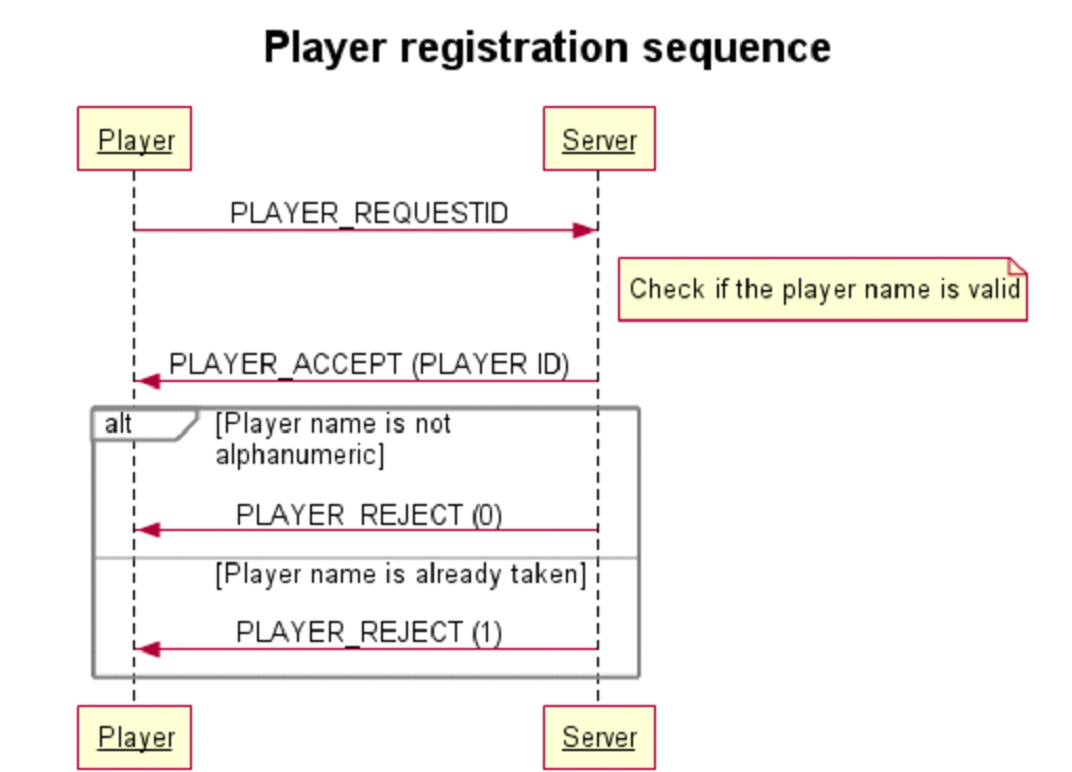
\includegraphics[scale=0.5]{registration-sequence}
\subsection*{Player is kicked from lobby}
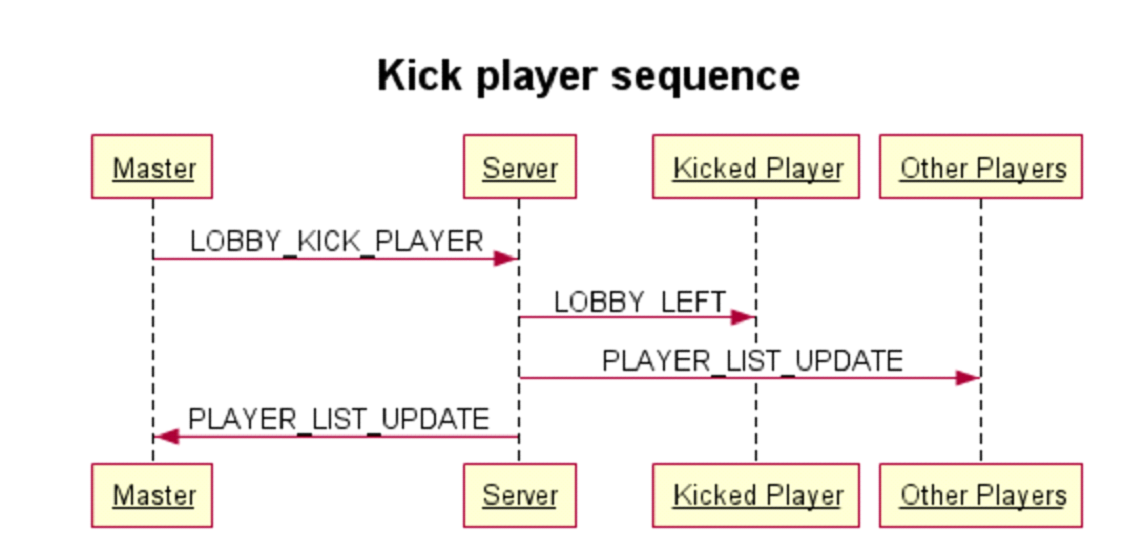
\includegraphics[scale=0.5]{kick_player_sequence}
\subsection*{Lobby creation}
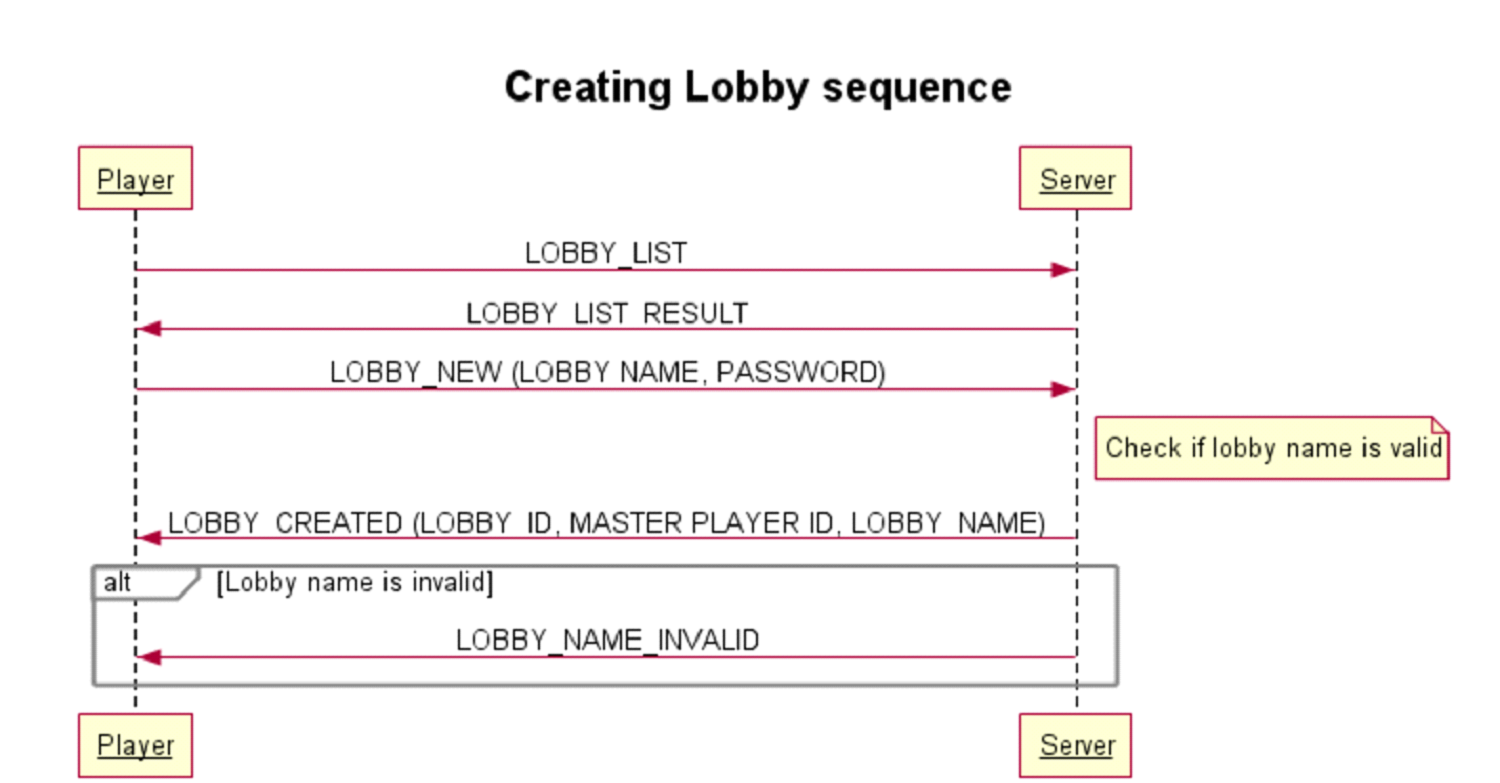
\includegraphics[scale=0.5]{lobby-creation-sequence}
\subsection*{Lobby joining}
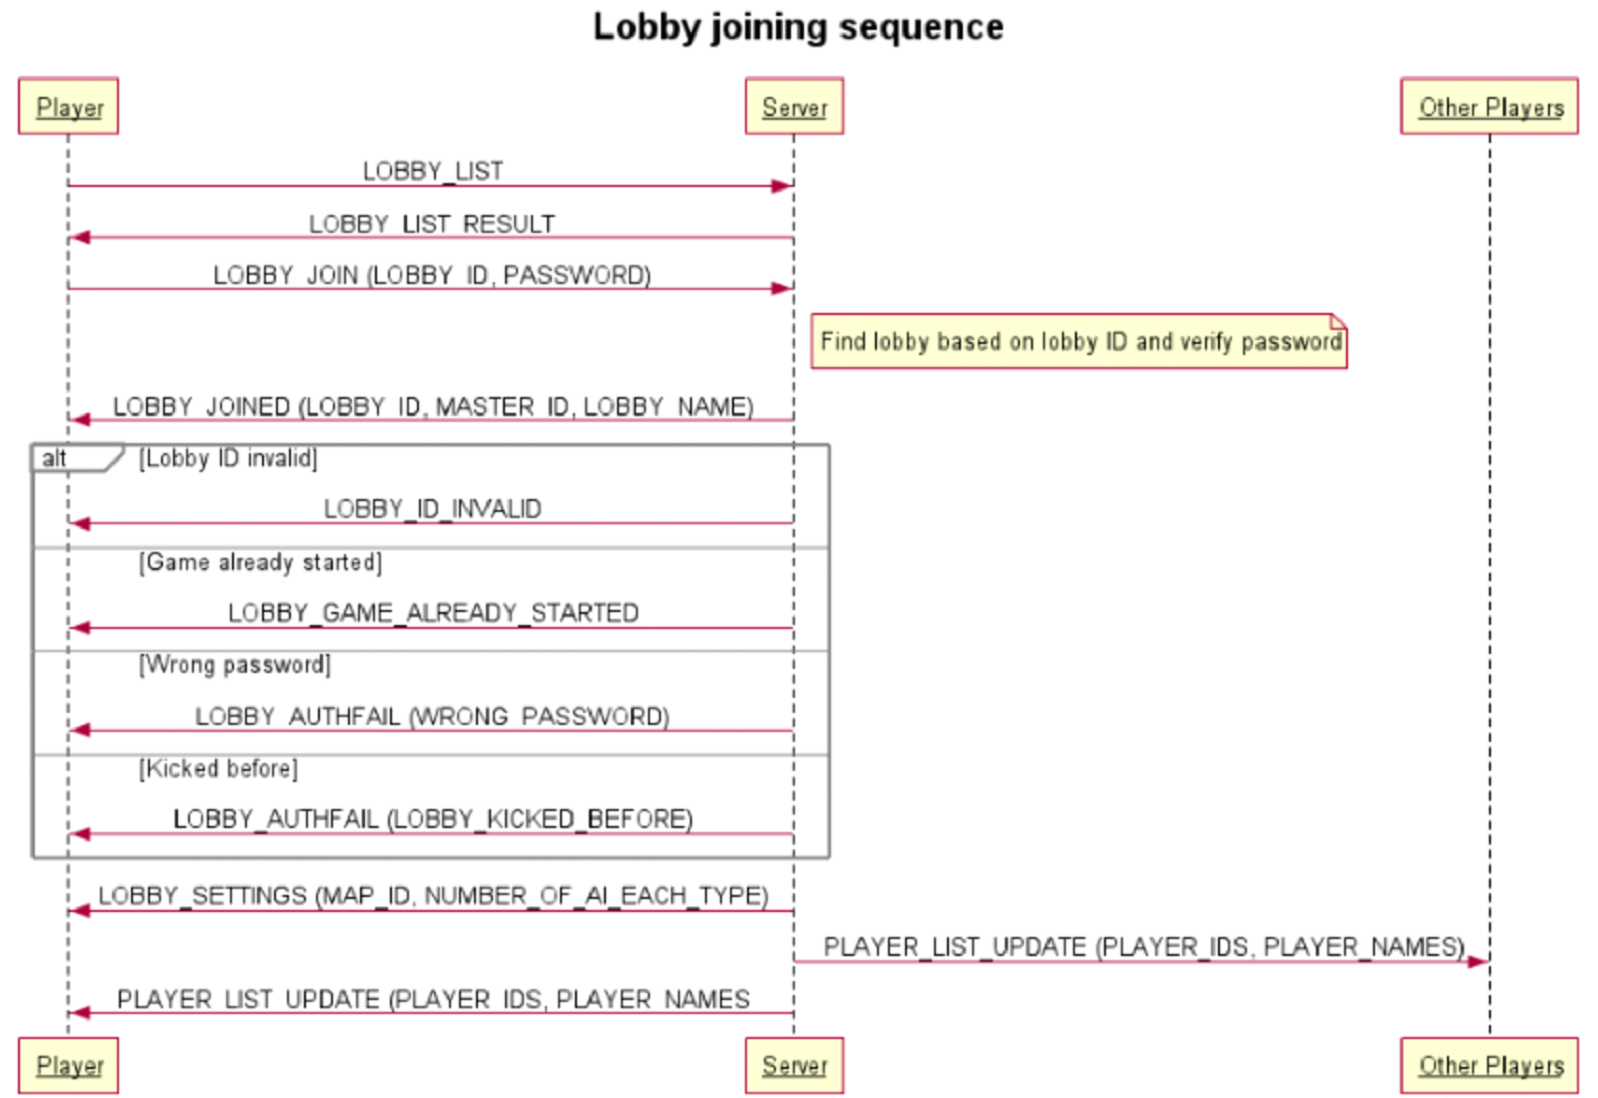
\includegraphics[scale=0.3]{lobby-join-sequence}
\subsection*{Lobby leaving}
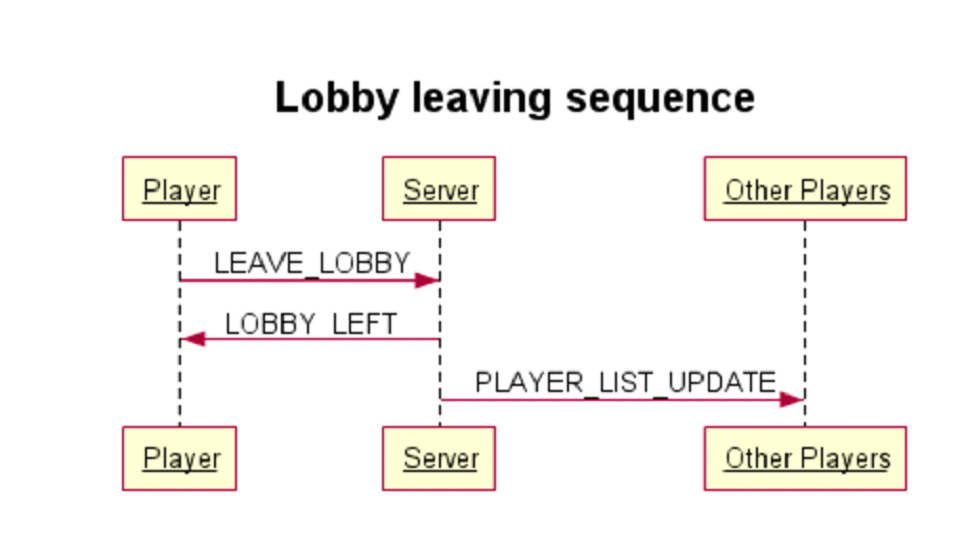
\includegraphics[scale=0.5]{lobby-leave-sequence}
\subsection*{Lobby messages}
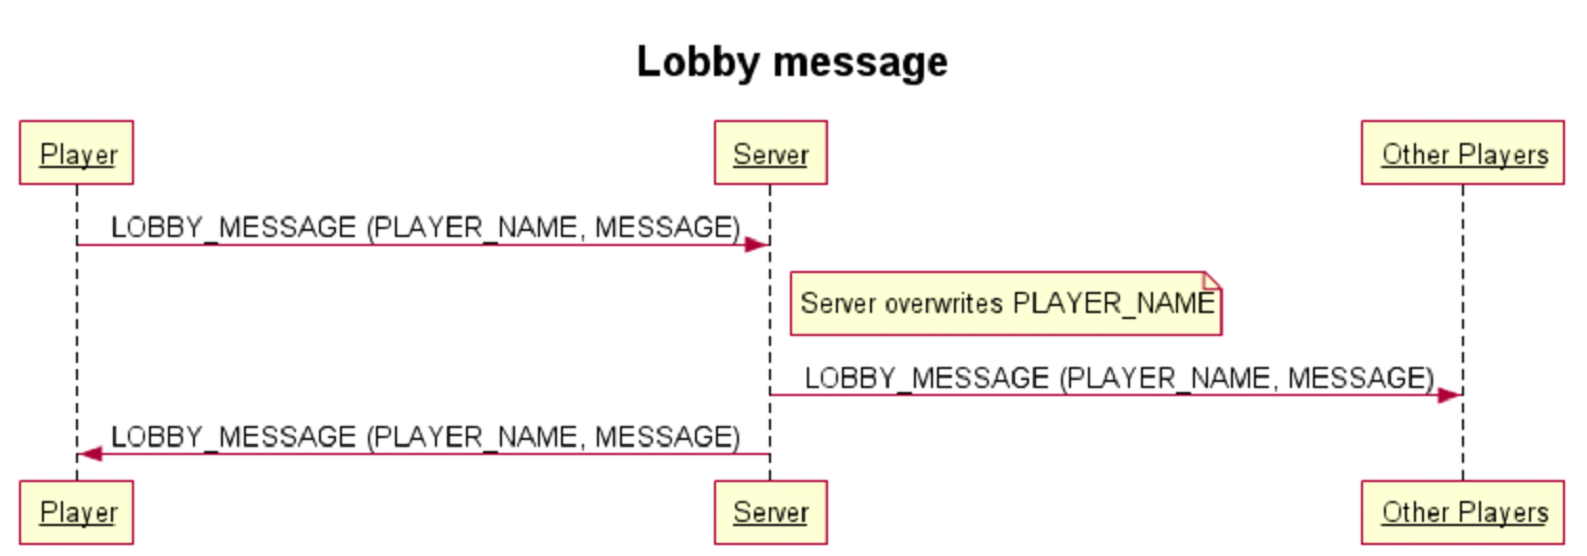
\includegraphics[scale=0.3]{lobby-message-sequence}
\subsection*{Lobby password changing}
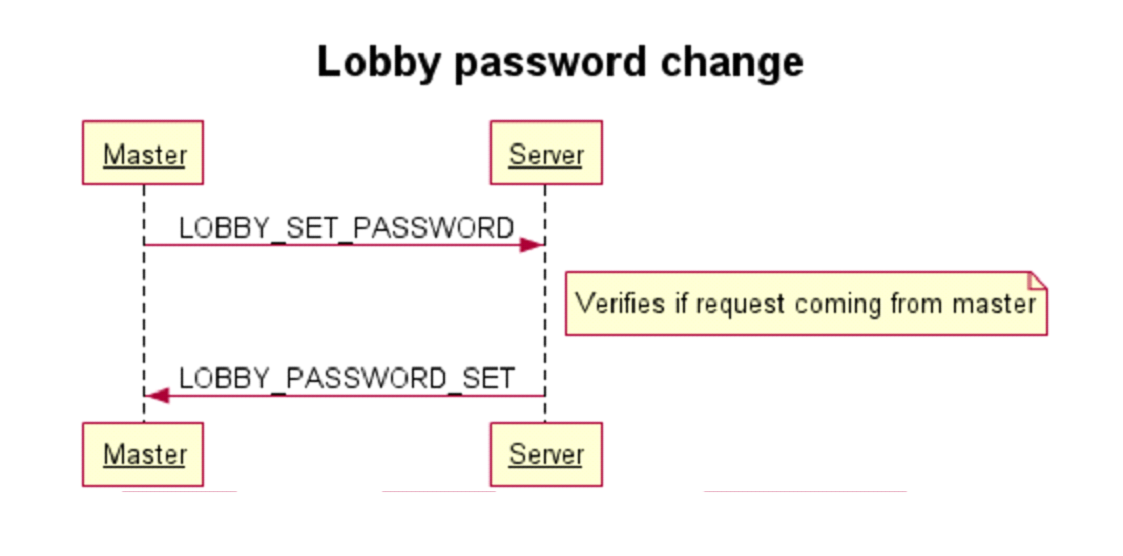
\includegraphics[scale=0.5]{lobby-password-sequence}
\subsection*{Lobby settings change}
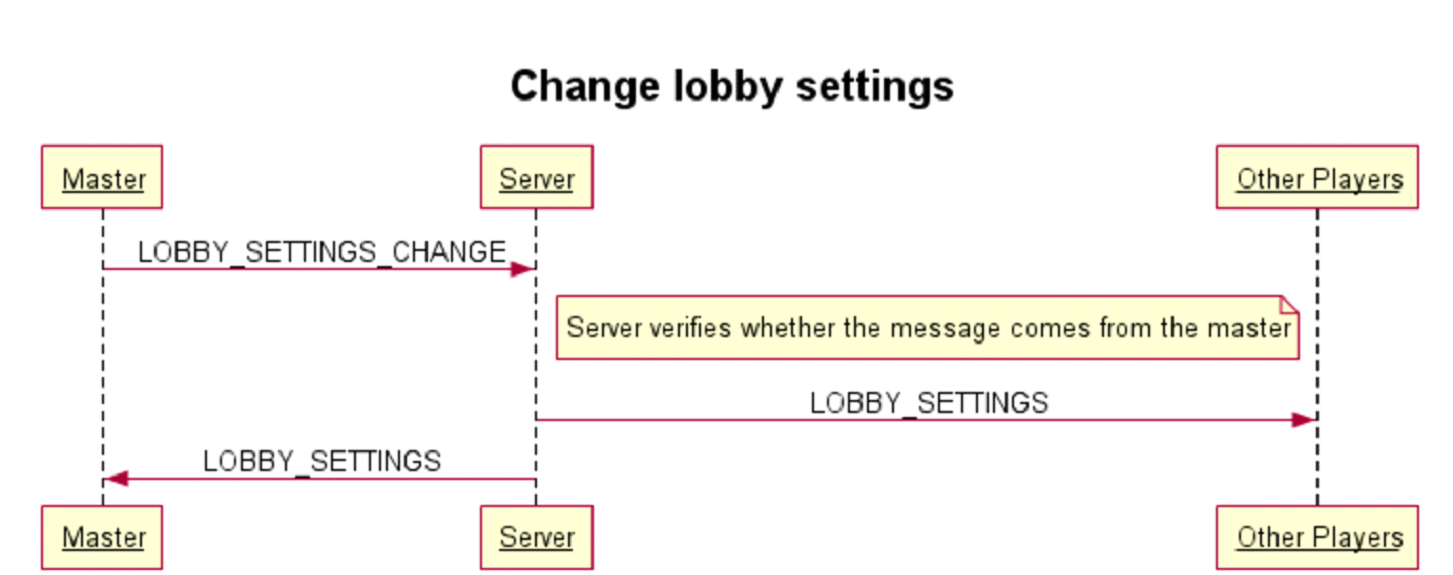
\includegraphics[scale=0.5]{lobby-settings-change-sequence}
\subsection*{Start and end game sequence}
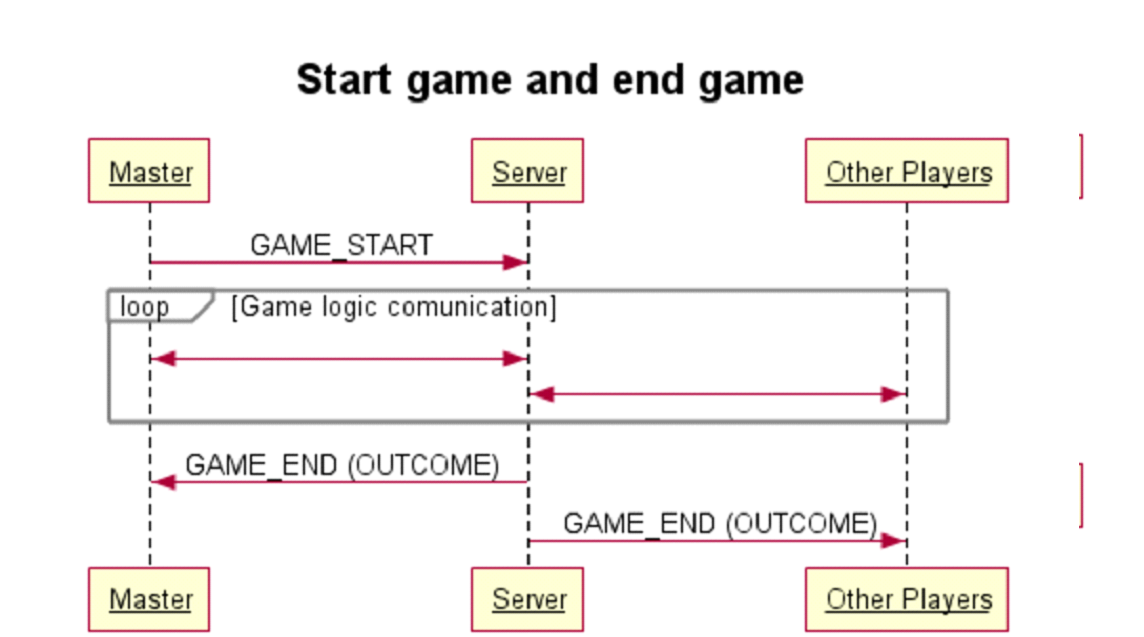
\includegraphics[scale=0.5]{start-end-sequence}
\subsection*{Unit throws grenade sequence}
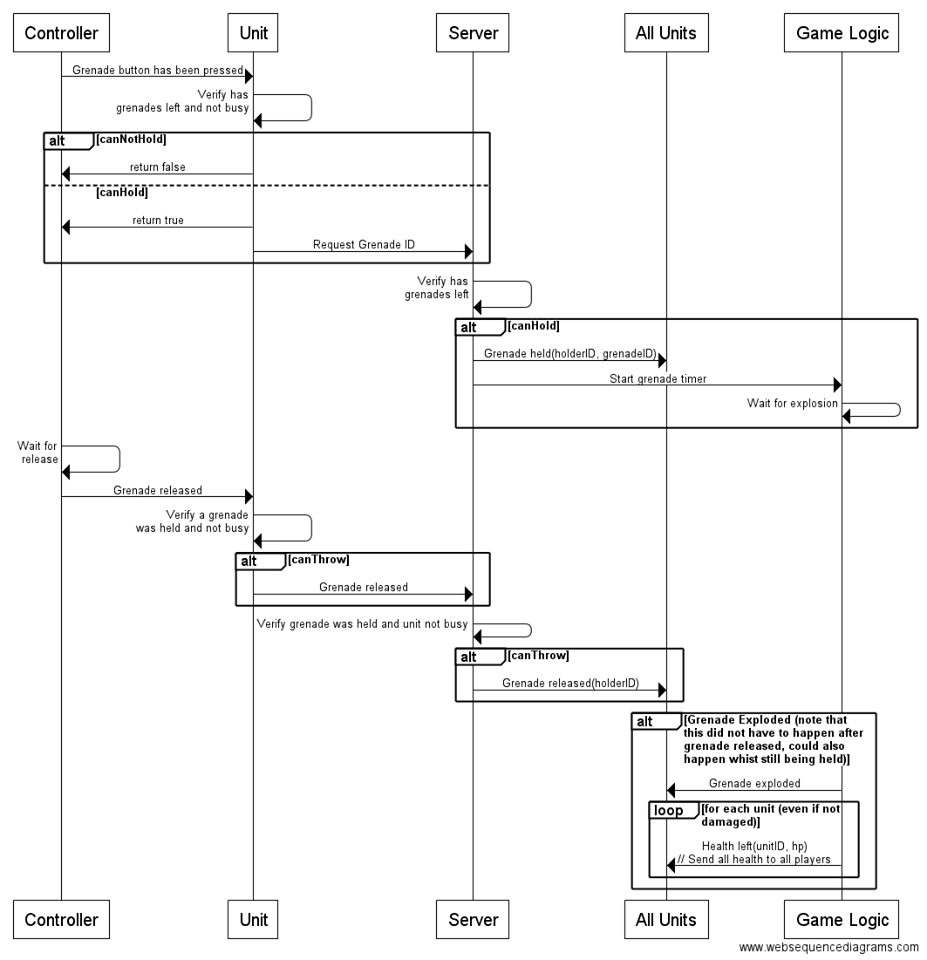
\includegraphics[scale=0.5]{grenade-sequence}
\newpage
\section{Appendix C: Use Case Descriptions}
This section details three use cases we documented for certain aspects of the game since the original specification.\return
\begin{tabularx}{\textwidth}{|l|X|} \hline
Name: & \textbf{Shoot a single bullet.} \\ \hline
ID: & UC1 \\ \hline
Description: & The process for firing a bullet when a User wants to shoot. \\ \hline
Actors: & User, Client, Server. \\ \hline
Frequency of use: & Very often. \\ \hline
Triggers: & The User presses the button/mouse click for which they expect a bullet to be fired. \\ \hline
Preconditions: & \begin{itemize}
\item The Client is connected to the Server and is in a game.
\item The User's unit is not currently 'busy' (reloading or throwing a grenade).
\item The User's unit is not dead.
\end{itemize} \\ \hline
Main Success Scenario: & \begin{enumerate}
\item The User presses the button/mouse clicks to shoot a bullet.
\item The Client sends a message to the server requesting a bullet ID (attaching their own unit ID).
\item The Server checks that the user can shoot at this time. This check involves making sure that they haven't shot too soon before (according to the weapon's rate of fire) and that they have a bullet in the magazine to fire.
\item If the  User's unit has a bullet to fire and it is not too soon since the last shot was fired, then the Server tells the requesting Client to fire the bullet and decrement the magazine by 1. The Server also tells all other Clients in the game to draw a bullet object according to the positions sent on their screens.
\end{enumerate} \\ \hline
Alternative Events: & \begin{enumerate}
\item If the User's unit does not have a bullet in the magazine to fire, do not fire a bullet and do not draw any bullets on other clients.
\item If the User's unit has fired too soon for the fire rate of the weapon, do not fire a bullet and do not draw any bullets on other clients.
\end{enumerate} \\ \hline
Postconditions: & \begin{itemize}
\item A moving bullet is rendered on all clients.
\item The magazine is depleted 1.
\end{itemize} \\ \hline
\end{tabularx}
\begin{tabularx}{\textwidth}{|l|X|} \hline
Name: & \textbf{Change the resolution of the client.} \\ \hline
ID: & UC2 \\ \hline
Description: & The process for a user changing the resolution of the client. \\ \hline
Actors: & User, Client. \\ \hline
Frequency of use: & Not too often. \\ \hline
Triggers: & The User feels like they need to change the resolution of their client (for a variety of reasons). \\ \hline
Preconditions: & \begin{itemize}
\item The User has the Client open.
\item The User is on the Client's main menu.
\end{itemize} \\ \hline
Main Success Scenario: & \begin{enumerate}
\item The User clicks on the 'Settings' button.
\item The User changes the resolution to their desired preference from the presets provided.
\item The User clicks on 'Apply changes' where the resolution is changed for the user.
\item The User is prompted with a dialog asking whether they want to keep the change or revert back. Doing nothing for 15 seconds will automatically revert.
\item The User clicks 'Keep'.
\end{enumerate} \\ \hline
Alternative Events: & \begin{enumerate}
\item The User could click 'Detect' instead of cycling through the presets so that a resolution can be suggested for the User based on their machine.
\item The User could click 'Revert' in which the resolution is changed back to its previous resolution.
\item The User could not click anything after clicking 'Apply changes' whereby after 15 seconds the Client automatically reverts the resolution back to what it was before.
\end{enumerate} \\ \hline
Postconditions: & \begin{itemize}
\item If 'Keep' is clicked on the dialog then the resolution of the Client is changed.
\item If 'Revert' or no action is made on the dialog then the resolution of the Client is not changed.
\end{itemize} \\ \hline
\end{tabularx}
\nl
\begin{tabularx}{\textwidth}{|l|X|} \hline
Name: & \textbf{Join a password protected lobby.} \\ \hline
ID: & UC3 \\ \hline
Description: & The process for a User trying to join a password protected lobby. \\ \hline
Actors: & User, Server, Client. \\ \hline
Frequency of use: & Often. \\ \hline
Triggers: & The User wants to join a private game. \\ \hline
Preconditions: & \begin{itemize}
\item The User is on the lobby list menu.
\item A password protected lobby is active on the Server and is not in-game nor full.
\item The User has not been kicked from the lobby previously.
\end{itemize} \\ \hline
Main Success Scenario: & \begin{enumerate}
\item The User clicks on the lobby they want to join on the Client and then clicks 'Join'.
\item The User should be presented with a dialog asking them to enter the password.
\item The User enters the correct password for the lobby.
\item The Server checks the password entered by the User.
\item The Server adds the User to the private lobby.
\end{enumerate} \\ \hline
Alternative Events: & \begin{enumerate}
\item The User enters an incorrect password into the dialog. The server sends a message to the Client informing that an incorrect password was entered. The Client displays a dialog to the User saying that the password is incorrect. Clicking 'Ok' should take the User back to the lobby list menu.
\end{enumerate} \\ \hline
Postconditions: & \begin{itemize}
\item If the password is correct, then the User is added to the lobby.
\item If the password is incorrect, the User is not added to the lobby and they are returned to the lobby list menu (after being displayed a dialog).
\end{itemize} \\ \hline
\end{tabularx}
\newpage
We also have the use case descriptions from the original specification.\return
\begin{tabularx}{\textwidth}{|l|X|} \hline
Use case name & \textbf{User login} \\ \hline
Description & The user wants to be able to connect to a server with a desired username and proceed to the main menu. \\ \hline
Primary actor(s) & The user \\ \hline
Secondary actor(s) & Client, Server \\ \hline
Triggering event & The game first opens. \\ \hline
Preconditions & The user is able to run the game. The user has an internet connection. \\ \hline
Postconditions & The user is connected to the server. \\ \hline
Main success scenario & 
\textbf{Goal:} User connected to user and enters main menu.
\begin{enumerate}[noitemsep,topsep=0px]
	\item The setup menu is displayed on the client.
	\item The user fills in their desired username, server details and connection method (UDP/TCP). 
	\item The user clicks the "Connect" button.
	\item The client sends a message to the server with this information.
	\item The server responds with a unique ID if the username was not already in use.
	\item The user is then presented with the main menu.
	\item The client requests a lobby list refresh from the server every 5 seconds, if the user is not currently in a game.
\end{enumerate} \\ \hline
Alternate flow & 
\textbf{Branching action:} The user missed a required field or has gave invalid input. \begin{enumerate}[noitemsep,topsep=0px,label={\arabic*}]
	\setcounter{enumi}{2} %use this to override numbering
	\item a. Prompt user to correct the form. Go to step 2.
\end{enumerate}
\textbf{Branching action:} Connection to server cannot be established. 
\begin{enumerate}[noitemsep,topsep=0px,label={\arabic*}]
	\setcounter{enumi}{3} %use this to override numbering
	\item a. The user is informed that the connection failed. Go to step 2.
\end{enumerate}
\textbf{Branching action:} Username was not unique. 
\begin{enumerate}[noitemsep,topsep=0px,label={\arabic*}]
	\setcounter{enumi}{4} %use this to override numbering
	\item a. The user is informed that the username was not unique. Go to step 2.
\end{enumerate}
\\ \hline
\end{tabularx}
$$$$
% New use case
\begin{tabularx}{\textwidth}{|l|X|} \hline
Use case name & \textbf{User creates lobby}\\ \hline
Description & The user wants to create a lobby so other players can join, ready to play a game. \\ \hline
Primary actor(s) & The user \\ \hline
Secondary actor(s) & Client, Server \\ \hline
Triggering event & The user clicks the "Create Lobby" button. \\ \hline
Preconditions & The user is connected to the server. \\ \hline
Postconditions & A lobby is created which other players can join, optionally with a password. \\ \hline
Main success scenario & 
\textbf{Goal:} User creates a lobby, optionally password-protected.
\begin{enumerate}[noitemsep,topsep=0px]
	\item The user is prompted for a name for the lobby and an optional password by the client. 
	\item The user enters a name and a password for the lobby.
	\item The client sends this information to the server.
	\item The server creates a lobby.
	\item The server sends the lobby ID back to the client.
	\item The client now refreshes the list of lobbies.
\end{enumerate} \\ \hline
Alternate flow & 
\textbf{Branching action:} The user has missed out the password field. 
\begin{enumerate}[noitemsep,topsep=0px,label={\arabic*}]
	\setcounter{enumi}{2} %use this to override numbering
	\item a. A lobby is created without a password. Go to step 4.
\end{enumerate}
\\ \hline
Exceptions &  
\textbf{Branching action:} Connection to the server is not present. 
\begin{enumerate}[noitemsep,topsep=0px,label={\arabic*}]
	\setcounter{enumi}{3} %use this to override numbering
	\item a. The user is informed that a connection is not present.
\end{enumerate}
\textbf{Branching action:} 	Lobby creation unsuccessful by server. 
\begin{enumerate}[noitemsep,topsep=0px,label={\arabic*}]
	\setcounter{enumi}{4} %use this to override numbering
	\item a. The user is informed that lobby creation was unsuccessful.
\end{enumerate} \\ \hline
\end{tabularx}
%end use case
$$$$
% New use case
\begin{tabularx}{\textwidth}{|l|X|} \hline
Use case name & \textbf{Unit throws grenade}\\ \hline
Description & When a unit throws a grenade, it explodes 5 seconds after. \\ \hline
Primary actor(s) & The unit who released the grenade\\ \hline
Secondary actor(s) & Another unit, Server \\ \hline
Triggering event & A unit throws a grenade. \\ \hline
Preconditions & The unit has at least 1 grenade. \\ \hline
Postconditions & The grenade has exploded. \\ \hline
Main success scenario & 
\textbf{Goal:} User joins their selected lobby.
\begin{enumerate}[noitemsep,topsep=0px]
	\item The grenade is released by a unit.
	\item The grenade travels in the direction is was released, eventually slowing to a stop due to friction. 
	\item After 5 seconds, the grenade explodes.
	\item Damage is applied to any surrounding units (depending on the distance they are from the grenade at the time of explosion) which are able to be damaged by the unit who released the grenade.
\end{enumerate} \\ \hline
Alternate flow & 
\textbf{Branching action:} Grenade collides with a wall or similar object. 
\begin{enumerate}[noitemsep,topsep=0px,label={\arabic*}]
	\setcounter{enumi}{1} %use this to override numbering
	\item a. The grenade is reflected.
\end{enumerate}
\textbf{Branching action:} Blast shield near explosion. 
\begin{enumerate}[noitemsep,topsep=0px,label={\arabic*}]
	\setcounter{enumi}{3} %use this to override numbering
	\item a. If a blast shield is between a unit and the explosion, the blast shield absorbs 80\% of the damage and the unit 20\% of the damage the unit would normally receive without the blast shield protecting it.
\end{enumerate}
\\ \hline
Exceptions &  
\textbf{Branching action:} Unit has no grenades. 
\begin{enumerate}[noitemsep,topsep=0px,label={\arabic*}]
	\setcounter{enumi}{1} %use this to override numbering
	\item a. No grenade is thrown.
\end{enumerate} \\ \hline
\end{tabularx}
\newpage
\section{Appendix D: Test Plan}
Due to timing constraints, it is not feasible for all features of our product to be tested with the same level of thoroughness. Thus, we will prioritise which features will require more coverage than others. This will provide a more rigorous testing strategy in which the most critical features of the system are tested more than others. Furthermore, more critical features of the product will be tested sooner than less critical features - this will allow the more critical features to be tested more and allow less room for implementation mistakes.\\
The following outlines the testing strategy for Escort The President and includes the following aspects:
\begin{enumerate}
\item Testing tools
\item Scope (Testing tasks)
\item Acceptance Criteria
\item List of JUnit Classes
\item Test Results
\end{enumerate}
\subsection{Testing Tools}
The software tool we used for the automated testing is JUnit and we aimed to build up a suite of regression tests using this tool which can be run when any new major functionality is added.\return
On top of this, we will also perform observation tests to verify that visual and audio functionality have been implemented in the expected manner; that certain noises are played at a particular time and animations are shown for expected motions. While this may seem subjective, it allows for greater a coverage as it is not trivial to test for concepts like atmosphere.\return
Cross testing (where members of the team write tests for parts of the system they may not directly have been involved in) should allow for a greater depth and quality of tests as well. A programmer will have a mental model and set of expectations of the flow through their work which may not be followed entirely by an outside user, so by having a variety of people (and therefore mental models) testing how something works should make it more robust in use.
\subsection{Scope}
Component and Integration Tests:
\begin{itemize}
\item Main menu (Settings, how to play, general navigation etc.)
\item Player Lobby
\item Game start (spawning of units, all players in game)
\item Movement of units (human and AI)
\item Weapons (shooting, switching, shield, grenades, AI shooting)
\item Powerups
\item Background music and sound snippets (e.g. gunfire)
\item Game end conditions (President dead or President safe)
\item Game restart
\item Cheat prevention
\end{itemize}
\subsection{Acceptance Criteria}
The acceptance criteria for the game is as follows:
\begin{itemize}
\item The user can connect to a server to play a game.
\item The user can set up their own server in order to play a game (connecting as localhost being an option).
\item The user can view how to play the game.
\item The user can view and change key bindings for the game.
\item The user can change their screen resolution.
\item The user can change music and sound levels for the game.
\item The user can mute music and sound levels for the game.
\item The user can disconnect from a server.
\item The user can view all available lobbies on the server.
\item The user can create a lobby (with or without a password).
\item The user can filter lobbies based on whether they are full, in-game, or private (or a mixture).
\item The user can join a lobby.
\item The owner of a lobby can specify the number of AI in game.
\item The owner of a lobby can specify the map.
\item The owner of a lobby can kick players from the lobby.
\item The user can have a chat message conversation with other players in the lobby and in game.
\item The user can access how to play and settings from a lobby.
\item The user should be kicked from a lobby if they are inactive for too long.
\item The user should be able to shoot in game at other units (including players).
\item The user should be able to throw grenades in game.
\item The user should be able to equip a shield.
\item The user should be able to switch the weapon they have equipped.
\item Users playing as assassins should be able to kill the president, resulting in an assassin victory.
\item Users playing as escorts should be able to escort the president to the saf zone.
\item The user should be able to pick up power-ups in game (subject to limits such as whether they already have maximum health, machine gun ammo or grenades).
\item The president can follow a particular unit when called upon to follow.
\end{itemize}
\subsection{Key Deliverables}
\begin{itemize}
\item Report on the project.
\item Game codebase.
\item Testing strategy.
\item JUnit test code (available in the Git repository) and results.
\item Inspection test plan and results.
\end{itemize}
\subsection{List of JUnit Classes and Test Results}
This test suite was built up throughout the duration of the project and were used to determine the correct running of the various aspects that are being tested. Test driven development was not one of the principles we followed but having these tests allowed us to continue checking that particular components worked after changes were made in other places (or to the logic of the component). If a test failed, it would then be a case of refining the logic of the program to make the test pass or by defining the test in a better way (that may capture some of the improvements made to the component).\return
The following is a list of all of the JUnit classes we used in the report. The results of the automated regression test suite we wrote in JUnit. These were carried  out on multiple machines to verify the integrity of the suite.
\subsubsection{Client Testing}
\begin{itemize}
\item client-test/src/escort/client/inputs/InputsTest.java (all passed)
\item client-test/src/escort/client/network/ServerConnectionTest.java (all passed)
\item client-test/src/escort/client/ui/components/ComponentsTest.java (all passed)
\item client-test/src/escort/client/ui/components/InputFieldTest.java (all passed)
\item client-test/src/escort/client/ui/components/ScrollableListTest.java (all passed)
\item client-test/src/escort/client/ui/components/StepperTest.java (all passed)
\item The client was mainly tested via an observation testing framework to be carried out by someone acting as a 'user' (See User Testing).
\end{itemize}
\subsubsection{User Testing}
\begin{itemize}
\item client-test/Observation-Testing/observation-tests.pdf (User testing framework).\return This includes results.
\end{itemize}
\subsubsection{Common Testing}
\begin{itemize}
\item common-test/src/escort/common/game/entities/EntityTest.java (all passed)
\item common-test/src/escort/common/game/entities/UnitTest.java (all passed)
\item common-test/src/escort/common/game/routePlanning/AStarSearchTest.java (all passed)
\item common-test/src/escort/common/game/routePlanning/NodeComparatorTest.java (all passed)
\item common-test/src/escort/common/game/routePlanning/NodeTest.java (all passed)
\item common-test/src/escort/common/game/routePlanning/PlanningMapTest.java (all passed)
\item common-test/src/escort/common/game/weapons/BlastShieldTest.java (all passed)
\item common-test/src/escort/common/game/weapons/GrenadeTest.java (all passed)
\item common-test/src/escort/common/game/powerups/ExtraGrenadesTest.java (all passed)
\item common-test/src/escort/common/game/powerups/ExtraMagsTest.java (all passed)
\item common-test/src/escort/common/game/powerups/ReplenishHealthTest.java (all passed)
\end{itemize}
\subsubsection{Server Testing}
\begin{itemize}
\item server-test/src/escort/server/game/ai/AILogicTest.java (all passed)
\item server-test/src/escort/server/game/ai/AICombatLogicTest.java (all passed)
\item server-test/src/escort/server/game/ai/AssassinControllerTest.java (all passed)
\item server-test/src/escort/server/game/ai/CivilianControllerTest.java (all passed)
\item server-test/src/escort/server/game/ai/EscortControllerTest.java (all passed)
\item server-test/src/escort/server/game/ai/PoliceControllerTest.java (all passed)
\item server-test/src/escort/server/game/ai/PresidentControllerTest.java (all passed)
\item server-test/src/escort/server/game/test/AssignmentTest.java
\item server-test/src/escort/server/game/test/EndGameTest.java (all passed)
\item server-test/src/escort/server/game/test/GameTest.java (all passed)
\item server-test/src/escort/server/game/test/SpawnTest.java (all passed)
\item server-test/src/escort/server/game/test/TraverseRoute.java (all passed)
\item server-test/src/escort/server/game/test/WeaponsTest.java (all passed)
\item server-test/src/escort/server/lobby/test/MoreLobbyTests.java (all passed)
\item server-test/src/escort/server/lobby/test/LobbyTest.java (all passed)
\item server-test/src/escort/server/network/test/ProtocolSwitchTest.java (all passed)
\item server-test/src/escort/server/network/test/ThrottleTest.java (all passed)
\end{itemize}
\newpage
\section{Appendix E: Risk Analysis}
The risk analysis from the SRS document.\return
\begin{tabularx}{\textwidth}{|p{4cm}|p{3cm}|X|} \hline
Risks & Likelihood & Methods to mitigate the risk \\ \hline
Members not understanding what they should be doing. & Likely towards the start of the project. & Have a discussion about all of the tasks that need to be carried out and assign them to people. Create a Gantt chart to help.\\ \hline
People falling behind on tasks. & Likely towards middle to the end of the project. & Try to make tasks well defined and make time estimates realistic. Build some slack in to the time.\\ \hline
Components not integrating easily. & Quite likely. & Spend more time on the design and on the interfaces in which components are intended to communicate via.\\ \hline
Duplication of work. & Quite unlikely. & If the tasks are well-defined and assigned accordingly then there should not be too much overlap.\\ \hline
People falling ill. & Unlikely. & Pick up other tasks while the person is ill. Hopefully it will not be severe and they will be able to do other tasks on return.\\ \hline
People not turning up for meetings. & Unlikely. & Seek assistance from the lecturer. May have to pick up other tasks on behalf of the missing person.\\ \hline
Some members doing more work than others. & Quite likely. & Try as best as possible to try and plan tasks so that the workload is balanced. If a task is unexpectedly short for someone then that person should seek out more tasks to help.\\ \hline
\end{tabularx}
\newpage
\section{Appendix F: Contribution tables}
Each member of the group has documented how much they think all other members (including themselves) have contributed to this project.
\subsection{Ahmed Bhallo}
\begin{tabular}{|c|c|} \hline
\textbf{Member name} & \textbf{Contribution ($\%$)}\\ \hline
Ahmed Bhallo & $20\%$ \\ \hline
James Birch & $20\%$ \\ \hline
Edward Dean & $20\%$ \\ \hline
Brendan Hart & $20\%$ \\ \hline
Kwong Hei Tsang & $20\%$ \\ \hline
\end{tabular}
\subsection{James Birch}
\begin{tabular}{|c|c|} \hline
\textbf{Member name} & \textbf{Contribution ($\%$)}\\ \hline
Ahmed Bhallo & $20\%$ \\ \hline
James Birch & $20\%$ \\ \hline
Edward Dean & $20\%$ \\ \hline
Brendan Hart & $20\%$ \\ \hline
Kwong Hei Tsang & $20\%$ \\ \hline
\end{tabular}
\subsection{Edward Dean}
\begin{tabular}{|c|c|} \hline
\textbf{Member name} & \textbf{Contribution ($\%$)}\\ \hline
Ahmed Bhallo & $20\%$ \\ \hline
James Birch & $20\%$ \\ \hline
Edward Dean & $20\%$ \\ \hline
Brendan Hart & $20\%$ \\ \hline
Kwong Hei Tsang & $20\%$ \\ \hline
\end{tabular}
\subsection{Brendan Hart}
\begin{tabular}{|c|c|} \hline
\textbf{Member name} & \textbf{Contribution ($\%$)}\\ \hline
Ahmed Bhallo & $20\%$ \\ \hline
James Birch & $20\%$ \\ \hline
Edward Dean & $20\%$ \\ \hline
Brendan Hart & $20\%$ \\ \hline
Kwong Hei Tsang & $20\%$ \\ \hline
\end{tabular}
\subsection{Kwong Hei Tsang}
\begin{tabular}{|c|c|} \hline
\textbf{Member name} & \textbf{Contribution ($\%$)}\\ \hline
Ahmed Bhallo & $20\%$ \\ \hline
James Birch & $20\%$ \\ \hline
Edward Dean & $20\%$ \\ \hline
Brendan Hart & $20\%$ \\ \hline
Kwong Hei Tsang & $20\%$ \\ \hline
\end{tabular}
\end{document}
